%%%%%%%%%%%%%%%%%%%%%%%%%%%%%%%%%%%%%%%%%%%%%%%%%%%%%%%%%%%%%%%%%%%%%%%%%%%%%%
%\vspace{-1ex}
\section{Evaluation} %Experimental Study
\label{sec-exp}
%%%%%%%%%%%%%%%%%%%%%%%%%%%%%%%%%%%%%%%%%%%%%%%%%%%%%%%%%%%%%%%%%%%%%%%%%%%%%%
In this section, we present extensive and systematic experimental studies and analyses of twelve representative \lsa algorithms.
Using three real-life datasets, we conduct five sets of tests to evaluate the effectiveness in terms of compression ratios and errors, efficiency (running time), aging friendliness and query friendliness of these representative algorithms using distance metrics \ped, \sed and \dad, and the impacts of error bounds $\epsilon$ and trajectory sizes.
%
%(1) the effectiveness of these algorithms, and
%(2) the efficiency of them.
%{An additional test of the effectiveness of near optimal algorithm (\nopts) is presented in Appendix B.}

%\vspace{-1ex}
\subsection{Experimental Setting}
%We first introduce the settings of our experimental study.

\stitle{Real-life Trajectory Datasets}.
We use three real-life datasets shown in \mytable{tab:datasets}, namely, Service car trajectory data (\ucar)~\cite{Lin:Cised}, Geolife trajectory data (\geolife)~\cite{Web:Geolife} and \mopsi trajectory data (\mopsi)~\cite{Web:Mopsi}, to evaluate those \lsa algorithms.
These data sets come from different sources, where \ucar is collected by cars in urban, and \geolife and \mopsi are a mixing of cars and individuals. They also have typical sampling rates used in practice, ranging from one point per second to one point per five seconds.
{The time interval between two neighbouring data points is occasionally very long, \eg greater than $10^7$ seconds.}
The data source and sampling rate also affect the performance of \lsa algorithms using certain distance metrics.

%\vspace{0.5ex}
\ni {(1) \ucar (also called ServiceCar in \cite{Lin:Cised}) is the GPS trajectories collected by a Chinese car rental company during Apr. 2015 to Nov. 2015. Most routes are located in big cities. The sampling rate is one point per $3$--$5$ seconds, and each trajectory has around $114.1K$ points.}
%.We randomly chose $1,000$ cars from them

%\vspace{0.5ex}
\ni {(2) \geolife is the GPS trajectories collected in the GeoLife project~\cite{Web:Geolife} by 182 users in a period from Apr. 2007 to Oct. 2011. These trajectories have a variety of sampling rates, among which 91\% are logged at one  point  per 1-5 seconds. The longest trajectory has 2,156,994 points.}

%\vspace{0.5ex}
\ni {(3) \mopsi is the GPS trajectories collected in the Mopsi project~\cite{Web:Mopsi} by 51 users in a period from 2008 to 2014. Most routes are located in Joensuu region, Finland. The sampling rate is one point per $2$ seconds, and each trajectory has around $153.9K$ points.}


\begin{table}[tb!]
	%\vspace{-1ex}
	\caption{\small Real-life trajectory datasets}
	\centering
	%\small
	\footnotesize
	\begin{tabular}{|l|c|c|c|c|}
		\hline
		\bf{Data sets}& \bf{Number\ of Trajectories}     &\bf{Sampling Rates (s)}   &\bf{Points~Per Trajectory}    &\bf{Total Points} \\	\hline
		%\taxi	&{500}	    &60	        &{$\sim42.8$K}      &{21.4M} \\	\hline
		%\truck	&10,368	    &1-60	    &$\sim71.9$     &746M \\	\hline
		%\ucar	&11,000	    &3-5	    &$\sim119.1$   &1.31G\\		\hline
		%
		\ucar \cite{Lin:Cised}	&{1000}	    &3-5	&$\sim114.0$K   &{114.0M} 	\\	\hline
		\geolife \cite{Web:Geolife}&182	    &1-5	&$\sim131.4$K   &24.2M	\\	\hline
		\mopsi \cite{Web:Mopsi}  &51	    	&2	    &$\sim153.9$K   &7.9M	\\	\hline
		%\act	& 10	    &1	    &$\sim11.8$    &112.8K	\\	\hline
	\end{tabular}
	\label{tab:datasets}
	\vspace{-2ex}
\end{table}


% \ni \emph{(1) Truck trajectory data} (\truck) is the GPS trajectories collected by \eat{10,368} trucks equipped with GPS sensors in China
% during a period from Mar. 2015 to Oct. 2015. The sampling rate varied from 1s to 60s.
%Trajectories mostly have around $50$ to $90$ thousand data points.



%\vspace{0.5ex}
%\ni \emph{(4) Act trajectory data} (\act) is a small set GPS trajectories collected with a high sampling rate of one point per second by our team members in 2017. There are 10 trajectories and each trajectory has around 11.8K points.

%The details of these datasets are shown in Table~\ref{tab:dataset}.

\stitle{Algorithms and implementation}.
We have implemented the representative algorithms shown in \mytable{tab:summary-lsa}.
 They are optimal algorithm \opt, batch algorithms \dpa and \tpa, online algorithms  \opwa, \bqsa, \squishe and {\dagots}, and one-pass algorithms  \operb, \siped, \cised, \intersec and \interval.
For one-pass algorithms \siped and \cised, we implement two versions of them (half and full $\epsilon$), denoted as \siped($\epsilon$), \siped($\frac{\epsilon}{2}$), \cised($\epsilon$) and \cised($\frac{\epsilon}{2}$).
%{The above algorithms all belong to strong simplification that output data points belong to the original trajectories.}
{Besides, algorithms \operb\cite{Lin:Operb} and \cised\cite{Lin:Cised} both have weak versions, named \operb-A and \cised-W, respectively.} %We also implement them.
For algorithm \cised, we fixed parameter $m=16$ as evaluated in \cite{Lin:Cised}, \ie 16-edges inscribe regular polygon.
For algorithm \operb, we remove its fifth optimization technique to make it fit for the definition of the {tolerance-zone error measure \cite{Daescu:metric,Barequet:3D,Chen:Space,Imai:Optimal,Melkman:Optimal} (otherwise, it is the \emph{infinite beam} error measure \cite{Daescu:metric,Chen:Space})}.
% For algorithm \nopts, we fixed parameter $m=32$.
All algorithms are implemented with Java.
{All tests are run on an x64-based  PC with 4 Intel(R) Core(TM) {i7-6700 CPU @3.40GHz} and 8GB of memory, and {the max heap size of Java VM is 4GB.}}
%, and each test was repeated over 3 times and the average is reported here.


We test these algorithms under varied error bounds $\epsilon$ and trajectory sizes, respectively. We first vary $\epsilon$ from $10m$ to $100m$ in \ped and \sed (or from $15^o$ to $90^o$ in \dad) on the entire four datasets, respectively. We then choose $10$ trajectories from each dataset, and vary the size \trajec{|T|} of a trajectory from $1,000$ points to $10,000$ points {(\ie from the first $1,000$ points to the first $10,000$ points of the trajectory)} while fixing the error bound $\epsilon=40$ metres or $\epsilon=45$ degrees.

\eat{%%%%%%%%%%%%%%%%%%%
	\stitle{Real-life Trajectory Datasets}.
	We use four real-life datasets shown in Table~\ref{tab:dataset} to test our solutions.
	
	\sstab{\bf(1) Taxi trajectory data}, referred to as \taxi, is the GPS trajectories collected by $12,727$ taxies equipped with GPS sensors in Beijing during a period
	from Nov. 1, 2010 to Nov. 30, 2010. The sampling rate was one point  per 60s, and \taxi has $39,100$ data points on average per trajectory.
	
	\sstab{\bf(2) Truck trajectory data}, referred to as \truck, is the GPS trajectories collected by 10,368 trucks equipped with GPS sensors in China
	during a period from Mar. 2015 to Oct. 2015. The sampling rate varied from 1s to 60s. Trajectories mostly have around $50$ to $90$ thousand data points.
	
	\sstab{\bf(3) Service car trajectory data}, referred to as \ucar,  is the GPS trajectories collected by a car rental company.
	We chose $11,000$ cars from them, during Apr. 2015 to Nov. 2015. The sampling rate was one point per $3$--$5$ seconds, and
	each trajectory has around $119.1K$ data points.
	
	{\sstab{\bf(4) GeoLife trajectory data}, referred to as \geolife, is the GPS trajectories collected in GeoLife project~\cite{Zheng:GeoLife} by 182 users in a period from Apr. 2007 to Oct. 2011. These trajectories have a variety of sampling rates, among which 91\% are logged in each 1-5 seconds or each 5-10 meters per point. The longest trajectory has 2,156,994 points.}
	%This dataset contains 182 trajectories, one trajectory for each user, with a total distance of about 1.2 million kilometers.
}%%%%%%%%%%%%%%%%%%%%%%%%%%%%%%%%%%%%%%%%%%%%%%%%%%%%%%%%%%%%%



\subsection{Evaluation Metrics}

{Compression ratios and errors are the most popular metrics to evaluate the effectiveness of \lsa algorithms, and they are also the measures to evaluate the aging friendliness of \lsa algorithms.
\myblue{Besides,} the running time  is used to evaluate the efficiency of \lsa algorithms.}

\stitle{Compression ratios.}
For trajectories $\{\dddot{\mathcal{T}_1}, \ldots, \dddot{\mathcal{T}_M}\}$ and their piece-wise line representations $\{\overline{\mathcal{T}_1}, \ldots, \overline{\mathcal{T}_M}\}$,
the compression ratio is $(\sum_{j=1}^{M} |\overline{\mathcal{T}}_j |)/(\sum_{j=1}^{M} |\dddot{\mathcal{T}}_j |)$.
By this definition, algorithms with lower compression ratios are better.

\stitle{Simplification errors.}
{The max (respectively average) simplification error is the max (respectively average) value of the distances from every point of the original trajectories to its representing line segment of the simplified trajectories.}


\eat{
Given a set of trajectories $\{\dddot{\mathcal{T}_1}, \ldots, \dddot{\mathcal{T}_M}\}$ and their piece-wise line representations
$\{\overline{\mathcal{T}_1}, \ldots, \overline{\mathcal{T}_M}\}$, and $P_{j,i}$ denoting
{one of the points} in trajectory $\dddot{\mathcal{T}}_j$ {represented by} a line segment $\mathcal{L}_{l,i}\in\overline{\mathcal{T}_l}$ ($l\in[1,M]$), then {the max error is $max\{d(P_{j,i}, \mathcal{L}_{l,i})\}$ for each i,j, l in [1, M],} and the average error is $\sum_{j=1}^{M}\sum_{i=0}^{M} d(P_{j,i}, \mathcal{L}_{l,i})/\sum_{j=1}^{M}{|\dddot{\mathcal{T}}_j |}$.
{Note that each point in the original trajectories are counted.}
\todo{Are the ranges of i,j, l correct?}}

\stitle{Running time.}
It is the efficiency of algorithms.
%We load and compress trajectories one by one, and only count the running time of the compressing process.


%%%%%%%%%%%%%%%%%%%%%%%%%%%%%%%%%%%%%%%%%%%%%%%%%%%%%%%%%%%%%%%%%%%%%%%%%%%%%%
\subsection{Experimental Results and Analyses}
%%%%%%%%%%%%%%%%%%%%%%%%%%%%%%%%%%%%%%%%%%%%%%%%%%%%%%%%%%%%%%%%%%%%%%%%%%%%%%
We next present our findings.




%%%%%%%%%%%%%%%%%%%%%%%%%%%%%%%%%%%%%%%%%%%%%%%%%%%%%%%%%%%%%%%%%%%%%%%%%%%%%
%\vspace{-1ex}
\subsubsection{Evaluation and \myblue{Analysis} of Compression Ratio}
%%%%%%%%%%%%%%%%%%%%%%%%%%%%%%%%%%%%%%%%%%%%%%%%%%%%%%%%%%%%%%%%%%%%%%%%

\eat{%%%%%%%
We first test the compression ratios of these algorithms under varied error bounds $\epsilon$ and trajectory sizes, respectively. We varied $\epsilon$ from $10m$ to $100m$ in \ped and \sed (or from $15^o$ to $90^o$ in \dad) on the entire four datasets, respectively. The results are reported in Figure~\ref{fig:cr-ped-epsilon}, Figure~\ref{fig:cr-sed-epsilon} and Figure~\ref{fig:cr-dad-epsilon} ({Note that the naive optimal algorithm using \sed or \dad is not reported here because it can not run with the full dataset as input}).
%
We then chose $10$ trajectories from each dataset \taxi, \ucar, \geolife and \mopsi, respectively, and varied the size \trajec{|T|} of a trajectory from $1,000$ points to $10,000$ points, while fixed error bound $\epsilon = 60$ meters for \ped and \sed ({or $\epsilon = 45$ degrees for \dad}).
The experimental results are reported in Figure~\ref{fig:cr-ped-size}, Figure~\ref{fig:cr-sed-size} and Figure~\ref{fig:cr-dad-size}.
}%%%%%%%%%%%

%We test the compression ratios of these algorithms under varied error bounds $\epsilon$ and trajectory sizes, respectively.
The compression ratios of these algorithms under varied error bounds $\epsilon$ and trajectory sizes are reported in Figures~\ref{fig:cr-ped-epsilon},~\ref{fig:cr-sed-epsilon},~\ref{fig:cr-dad-epsilon},~\ref{fig:cr-ped-size},~\ref{fig:cr-sed-size} and~\ref{fig:cr-dad-size}.
{Note that the optimal algorithm using \sed and \dad is not reported in Figures~\ref{fig:cr-ped-epsilon},~\ref{fig:cr-sed-epsilon} and~\ref{fig:cr-dad-epsilon} as it runs out of memory when compressing the full dataset}. We first report our findings.

\begin{figure*}[tb!]
	\centering
	%\includegraphics[scale=0.250]{Figures/Exp-PED-CR-epsilon-taxi.jpg}\hspace{0.5ex}
	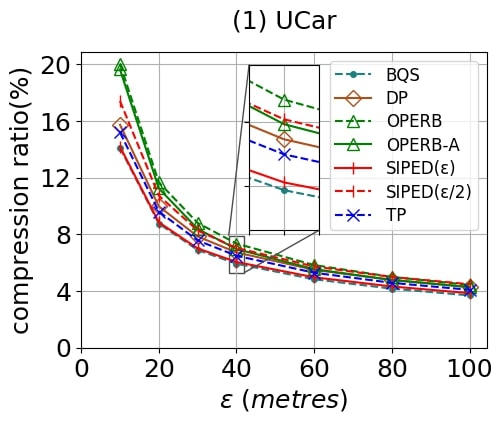
\includegraphics[scale=0.250]{Figures/Exp-PED-CR-epsilon-service.jpg} 	\hspace{0.5ex}
	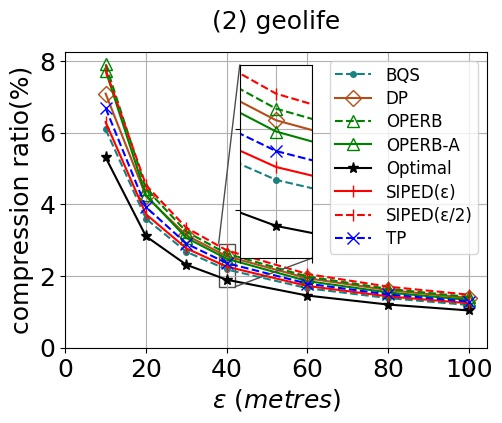
\includegraphics[scale=0.348]{Figures/Exp-PED-CR-epsilon-geolife.jpg}	\hspace{0.5ex}
	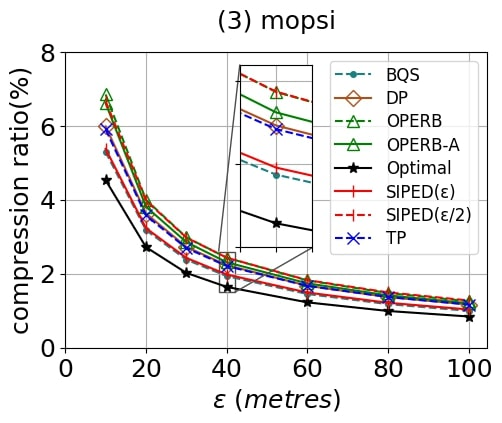
\includegraphics[scale=0.250]{Figures/Exp-PED-CR-epsilon-mopsi.jpg}		
	\vspace{-2ex}
	\caption{\small Evaluation of compression ratios (\ped) on full datasets: varying the error bound $\epsilon$.}
	\label{fig:cr-ped-epsilon}
	\vspace{-2ex}
\end{figure*}
\begin{figure*}[tb!]
	\centering
	%\includegraphics[scale=0.250]{Figures/Exp-SED-CR-epsilon-taxi.jpg}\hspace{0.5ex}
	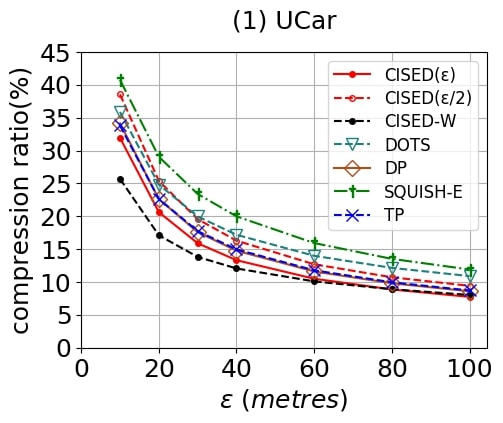
\includegraphics[scale=0.250]{Figures/Exp-SED-CR-epsilon-service.jpg} 	\hspace{0.5ex}
	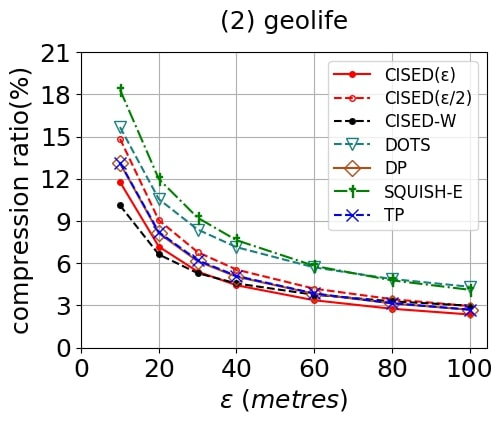
\includegraphics[scale=0.250]{Figures/Exp-SED-CR-epsilon-geolife.jpg}	\hspace{0.5ex}
	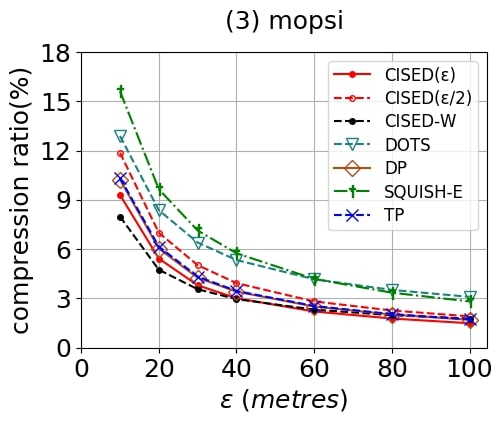
\includegraphics[scale=0.250]{Figures/Exp-SED-CR-epsilon-mopsi.jpg}		
	\vspace{-2ex}
	\caption{\small Evaluation of compression ratios (\sed) on full datasets: varying the error bound $\epsilon$.}
	\label{fig:cr-sed-epsilon}
	\vspace{-2ex}
\end{figure*}
\begin{figure*}[tb!]
	\centering
	%\includegraphics[scale=0.250]{Figures/Exp-DAD-CR-epsilon-taxi.jpg}\hspace{0.5ex}
	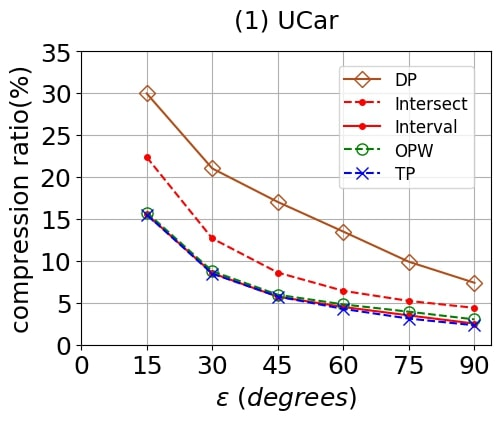
\includegraphics[scale=0.250]{Figures/Exp-DAD-CR-epsilon-service.jpg} 	\hspace{0.5ex}
	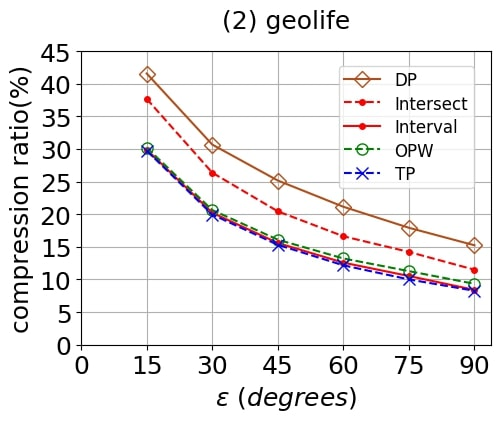
\includegraphics[scale=0.250]{Figures/Exp-DAD-CR-epsilon-geolife.jpg}	\hspace{0.5ex}
	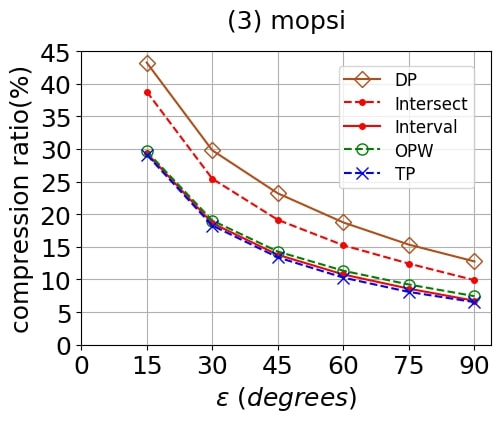
\includegraphics[scale=0.250]{Figures/Exp-DAD-CR-epsilon-mopsi.jpg}		
	\vspace{-2ex}
	\caption{\small Evaluation of compression ratios (\dad) on full datasets: varying the error bound $\epsilon$.}
	\label{fig:cr-dad-epsilon}
	\vspace{-2ex}
\end{figure*}


%%%%%%%%%%%%%%%%%
\sstab(1)  {Datasets may have impacts on the compression ratios of \lsa algorithms. Datasets with higher sampling rates typically have better compression ratios for \ped and \sed, while it is opposite for \dad. {When using \dad, the} dataset collected by cars (\eg~\ucar) has better compression ratios than the datasets partially collected by individuals (\eg~\geolife and \mopsi), as cars typically move more regularly than individuals {in directions}.}
%{otherwise, it has poorer compression ratios than \geolife and \mopsi, partially because cars have a broad range of speed and they frequently stop because of traffic light}

\sstab(2) {Compression ratios are insensitive to the sizes of trajectories.} {The reason lies in that once the distance is greater than the error bound, a line segment is produced, and the compression continues to repeat this process, which is essentially irrelevant to the sizes of trajectories. This is also the key to preserve the error bound for any of the optimal, batch, online and one-pass algorithms.}

\sstab(3) The compression ratios of algorithms using \ped from the best
to the worst are normally the optimal algorithm \opt, online algorithm \bqsa, one-pass algorithm \siped($\epsilon$), batch algorithms \tpa and \dpa and one-pass algorithm {\operb-A}, and one-pass algorithms \siped($\frac{\epsilon}{2}$) and \operb.
The output sizes of algorithms \bqsa and \siped({$\epsilon$}) are on average
($113.32\%$, $120.22\%$, $120.83\%$) and ($116.04\%$, $124.46\%$, $124.24\%$) of algorithm \opt
on datasets \dSets, respectively.
Algorithms \tpa, \dpa and {\operb-A} are comparable, and their output sizes are on average
($125.05\%$, $131.01\%$, $138.01\%$), ($130.03\%$, $140.56\%$, $139.00\%$) and {( $134.16\%$, $137.73\%$, $144.31\%$)} of \opt
on datasets \dSets, respectively.
Algorithms \siped($\frac{\epsilon}{2}$) and \operb are comparable, and they are on average
($136.73\%$, $150.23\%$, $152.29\%$) and ($143.14\%$, $147.80\%$, $152.37\%$) of \opt on datasets \dSets, respectively.
%
For example, in \mopsi, the compression ratios of algorithms
(\opt, \tpa, \dpa, \bqsa, \siped(${\epsilon}$), \siped($\frac{\epsilon}{2}$), \operb, {\operb-A} ) are ($1.6\%$, $2.2\%$, $2.2\%$, $1.9\%$, $2.0\%$, $2.4\%$, $2.4\%$, {$2.3\%$}) when $\epsilon$ = $40m$.
%
\begin{figure*}[tb!]
	\centering
	%\includegraphics[scale=0.250]{Figures/Exp-PED-CR-size-taxi.jpg}\hspace{0.5ex}
	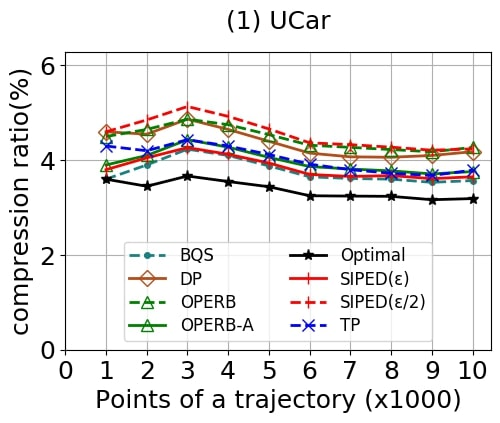
\includegraphics[scale=0.250]{Figures/Exp-PED-CR-size-service.jpg} 	\hspace{0.5ex}
	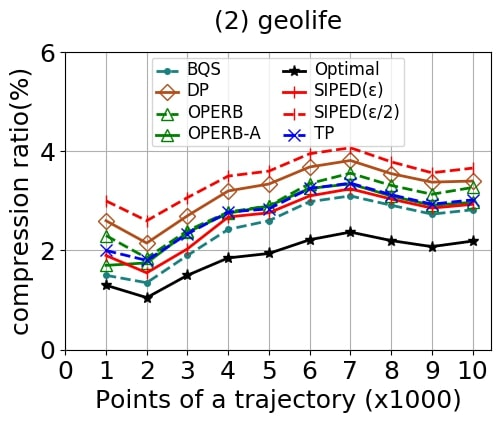
\includegraphics[scale=0.250]{Figures/Exp-PED-CR-size-geolife.jpg}	\hspace{0.5ex}
	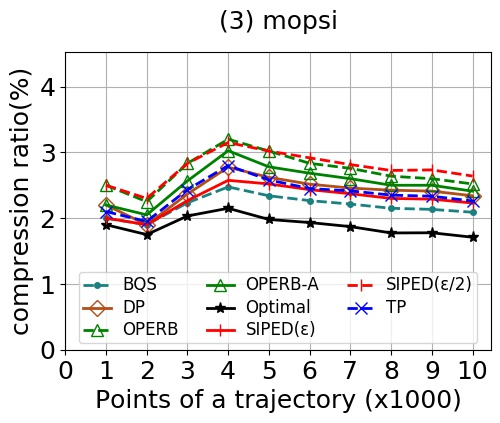
\includegraphics[scale=0.348]{Figures/Exp-PED-CR-size-mopsi.jpg}		
	\vspace{-2ex}
	\caption{\small Evaluation of compression ratios (\ped) on small datasets: varying the size of
		trajectories.}
	\label{fig:cr-ped-size}
	\vspace{-2ex}
\end{figure*}
\begin{figure*}[tb!]
	\centering
	%\includegraphics[scale=0.250]{Figures/Exp-SED-CR-size-taxi.jpg}\hspace{0.5ex}
	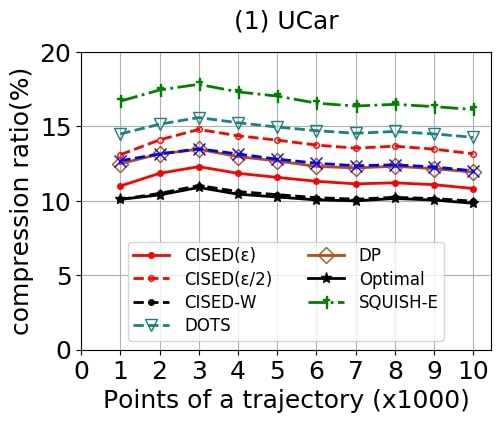
\includegraphics[scale=0.250]{Figures/Exp-SED-CR-size-service.jpg} 	\hspace{0.5ex}
	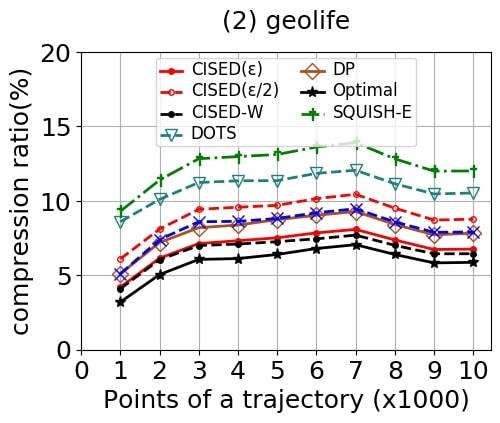
\includegraphics[scale=0.250]{Figures/Exp-SED-CR-size-geolife.jpg}	\hspace{0.5ex}
	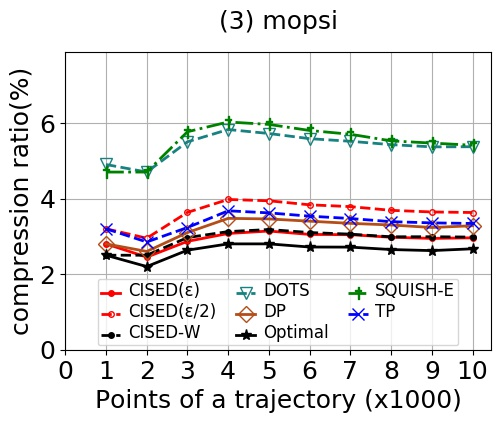
\includegraphics[scale=0.348]{Figures/Exp-SED-CR-size-mopsi.jpg}		
	\vspace{-2ex}
	\caption{\small Evaluation of compression ratios (\sed) on small datasets: varying the size of
		trajectories.}
	\label{fig:cr-sed-size}
	\vspace{-2ex}
\end{figure*}
\begin{figure*}[tb!]
	\centering
	%\includegraphics[scale=0.50]{Figures/Exp-DAD-CR-size-taxi.jpg}\hspace{0.5ex}
	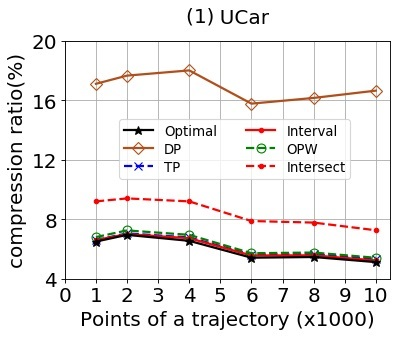
\includegraphics[scale=0.52]{Figures/Exp-DAD-CR-size-service.jpg} 	\hspace{0.5ex}
	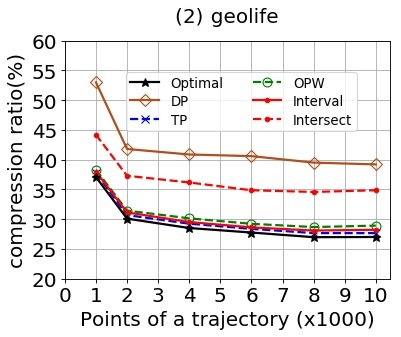
\includegraphics[scale=0.52]{Figures/Exp-DAD-CR-size-geolife.jpg}	\hspace{0.5ex}
	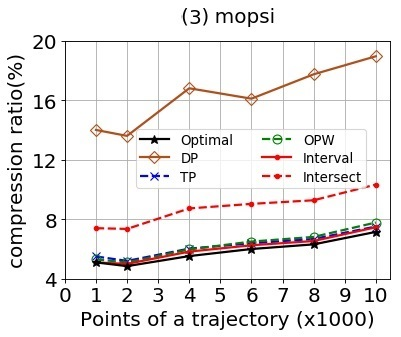
\includegraphics[scale=0.52]{Figures/Exp-DAD-CR-size-mopsi.jpg}		
	\vspace{-2ex}
	\caption{\small Evaluation of compression ratios (\dad) on small datasets: varying the size of trajectories.}
	\label{fig:cr-dad-size}
	\vspace{-2ex}
\end{figure*}




%%%%%%%%%%%%%%%%%
\sstab(4) The compression ratios of algorithms using \sed from the best
to the worst are normally the \opt algorithm, one-pass algorithms {\cised-W} and \cised($\epsilon$), batch algorithms \tpa and
\dpa, one-pass algorithm \cised($\frac{\epsilon}{2}$), and online algorithm {\dagots} and \squishe.
%
{Algorithms \tpa and \dpa are comparable, and they are on average
($125.23\%$, $143.92\%$, $128.63\%$) and ($123.93\%$, $141.46\%$, $121.14\%$)
 of algorithm \opt on datasets \dSets, respectively.}
%
{Algorithms {\cised-W}, \cised(${\epsilon}$), \cised($\frac{\epsilon}{2}$), \squishe and {\dagots} are on average {($100.98\%, 108.16\%, 110.15\%$)}, ($109.27\%$, $110.13\%$, $115.90\%$,), ($134.35\%$, $159.30\%$, $136.06\%$), ($165.94\%$, $225.68\%$, $206.90\%$) and {$(140.98\%, 200.36\%, 198.73\%)$}
 of \opt on \dSets, respectively.}
%
For example, in \mopsi, the compression ratios of algorithms
(\tpa, \dpa, \squishe, {\dagots}, \cised(${\epsilon}$), \cised($\frac{\epsilon}{2}$),  {\cised-W})
are ($3.45\%$, $3.41\%$, $5.75\%$, {$5.34\%$}, $3.02\%$, $3.86\%$,  {$2.96\%$}), respectively, when $\epsilon$ = $40m$.
%
%Algorithms \tpa and \dpa are comparable, and they are on average ($122.69\%$, $129.08\%$, $131.97\%$, $131.01\%$) and ($121.36\%$, $129.27\%$, $130.11\%$, $126.21\%$) of the near optimal algorithm \nopts on datasets \dSets, respectively.
%Algorithms \cised and \squishe are on average ($132.07\%$, $139.67\%$, $146.56\%$, $135.10\%$) and ($164.47\%$, $189.87\%$, $213.30\%$, $186.72\%$) of \nopts on datasets \dSets, respectively.
%
%For example, in \mopsi, the compression ratios of algorithms (\nopts, \tpa, \dpa, \squishe, \cised) are ($2.62\%$, $3.45\%$, $3.41\%$, $5.75\%$, $3.86\%$), respectively, when $\epsilon$ = $40m$.
%

%%%%%%%%%%%%%%%%%
\sstab(5) The compression ratios of algorithms using \dad from the best
to the worst are the \opt algorithm, batch algorithm \tpa and
one-pass algorithm \interval, online algorithm \opwa, one-pass algorithm \intersec and batch algorithm \dpa.
%
{Algorithms \tpa, \opwa and \interval are comparable, and are on average
($102.91\%$, $102.27\%$, $106.88\%$), ($116.09\%$, $107.11\%$, $115.42\%$) and ($101.98\%$, $103.52\%$, $103.43\%$)
 of algorithm \opt on datasets \dSets, respectively.}
%
{Algorithms \intersec and \dpa are on average ($156.00\%$, $121.20\%$, $230.52\%$) and ($283.93\%$, $143.79\%$, $278.89\%$)
 of algorithm \opt on datasets \dSets, respectively.}
%
For example, in \mopsi, the compression ratios of algorithms (\tpa, \dpa, \opwa, \interval, \intersec)
are ($13.3\%$, $23.1\%$, $14.12\%$, $13.7\%$, $18.96\%$), respectively, when $\epsilon$ = $45$ degrees.
%






We then present analyses from the views of \lsa algorithms and distance metrics.


\stitle{Analyses of \lsa algorithms}. The \opt algorithm is the best in terms of compression ratios, followed by online algorithms \opwa and \bqsa and one-pass algorithms using the full $\epsilon$ \emph{sector/cone/range}. One-pass algorithms using a half $\epsilon$ \emph{sector/cone/range} and batch algorithms except \dpa using \dad also have good compression ratios.
\eat{
 are the most outstanding algorithms among all sub optimal algorithms.
, followed by batch algorithms. Online algorithms have varied compression ratios, ranging from the worst to the similar with batch and one-pass algorithms.
}



%\todo{Batch: Bottom-up vs Top-down.}
For batch algorithms, bottom-up algorithm (\tpa) and top-down algorithm (\dpa) have the similar compression ratios when using \ped and \sed. However, when using \dad, bottom-up methods have obviously better compression ratios than top-down methods.  As we know that top-down algorithms split a long trajectory $[P_s, ..., P_e]$ into two sub-trajectories by finding out a splitting point $P_i (s<i<e)$ that has the max position deviation (or whose line segment $\vv{P_{i-1}P_{i}}$ has the max direction deviation) to line segment $\vv{P_sP_{e}}$. Though this strategy works well with \ped and \sed, a point with the max direction deviation may not be a reasonable splitting point in the direction-aware scenario. Thus it leads to a poorer compression ratio. However, bottom-up methods do not have this weakness as they always merge neighbouring points.



%\todo{Online: }
For online algorithms, \bqsa and \opwa are comparable with the best sub-optimal algorithms. This is because \opwa is indeed a combination of \dpa and opening window, and \bqsa is mainly an efficiency optimized \opwa.
\squishe has the poorest compression ratio among all algorithms using \sed. This is the result of its mechanism: \squishe estimates the lowest \sed error and removes the point with ``predicted to introduce the lowest amount of error into the compression'' \cite{Muckell:SQUISH}. Its ``prediction'' method is not accurate enough, thus, in order to ensure the error bound, it may ignore too many potential points that could be represented by a line segment. {\dagots~also shows poor compression ratios in these tests. This is related to \lissed, a cumulative error measure that \dagots~uses, in which each point contributes to the error, such that the \lissed error bound of $\epsilon^2$ may limit this algorithm to compress more points into a line segment, while those points may be compressed \wrt the  \sed error bound of $\epsilon$.}

%\todo{One pass: half $\epsilon$ vs full $\epsilon$.}
For one-pass algorithms, the full $\epsilon$ sector/cone/range combining with a position/direction constraint always has better compression ratios than the half $\epsilon$ sector/cone/range versions in all datasets, and they are comparable with the best sub-optimal algorithms.
This may be related to the moving habits or patterns of moving objects that are implied in trajectories.
That is, a moving object, like an individual or a car, usually keeps moving forward for quite a long time, engendering a sequence of data points distributing in a narrow strip. Under such circumstance, a new data point is quite possibly living in the common intersection of larger sectors/cones/ranges, which further leads to a better compression ratio.
%which lets more data points be represented by a result line segment.

{Moreover, weak algorithms \operb-A and \cised-W typically have a few advantages in terms of compression ratios compared with their strong simplification counterparts \operb and \cised for the cases with relatively small error bounds (\eg $\epsilon<40$ meters in these tests).}




\stitle{Analyses of distance metrics}.
Though \ped, \sed and \dad are different distances, the comparison of their compression ratios is helpful to choose an effective distance metric.
%whose usages are mainly decided by application requirements
%
First,  given the same error bound $\epsilon$, the compression ratios of algorithms using \ped are obviously better
than using \sed.
{This is because \sed saves temporal information while \ped does not}.
More specifically, \emph{the output sizes of using \sed are approximately twice of \ped.}
%
As shown in Figures~\ref{fig:cr-ped-epsilon} and~\ref{fig:cr-sed-epsilon}, the output sizes of algorithms \tpa and \dpa
using \ped are on average ($43.55\%$, $47.49\%$, $63.15\%$) and ($45.79\%$,
$50.88\%$, $64.50\%$) of algorithms \tpa and \dpa using \sed on datasets \dSets, respectively.
%
%and in Figure~\ref{fig:cr-ped-size} and Figure~\ref{fig:cr-sed-size}, the compression ratios of algorithms \opt, \tpa and \dpa using \ped are on average {($56.03\%$, $33.42\%$, $33.12\%$, $72.42\%$),	($55.78\%$, $31.88\%$, $34.27\%$, $69.44\%$) and ($58.09\%$, $34.82\%$,	$40.91\%$, $75.06\%$)} of algorithms \opt, \tpa and \dpa using \sed on datasets \dSets, respectively.
%
This result shows ~\sed saves temporal information at a price of twice more data points. {Although the loss of temporal information may lead to unexpected results, \eg unbounded answer-errors to spatio-temporal queries (see Section \ref{sec-exp-query}), this price is worthwhile for certain applications. }


Secondly, {we find that \sed has obviously better compression ratios than \dad on datasets \geolife and \mopsi, and a bit poorer than \dad in \ucar.}
This is because some \geolife and \mopsi trajectories are collected by individuals that are in transportation modes of walking, running and riding, and moving objects in those modes may change their directions with a considerable range (\eg large than $60$ degrees) more frequently than cars in urban. Moreover, \geolife and \mopsi have higher sampling rates than \ucar, which capture more direction changes, \ie direction changes in a small time interval.
%
{Indeed, it is hard to compare \sed and \dad under absolutely fair conditions, as \sed is a Euclidean distance metric, having a value in $[0, \infty]$ meters, and DAD is a direction metric,  having a value in $[0,360)$ degrees. Hence, we choose to consider more practical scenarios, \ie one uses \sed with $\epsilon  \le  100$ meters, and the other uses \dad with $\epsilon \le 60$ degrees, and we compare the performance of \sed with $\epsilon=100/k$ meters \emph{vs.} \dad with $\epsilon=60/k$ degrees with $k \ge 1$. We also follow this when comparing \sed and \dad in the sequel.}
%It seems that it is a normal phenomenon that a moving object frequently changes its direction with a considerable range (\eg large than $60$ degrees) during a trip.



\eat{
	
	\sstab (1) Trajectory sizes have few impacts on compression ratios.
	
	\sstab (1) When increasing $\epsilon$, the compression ratios decrease.
	%For example, in \mopsi, the compression ratios are greater than {$4\%$} when $\epsilon$ = $10m$, and less than {$2\%$} when $\epsilon$ = $100m$.
	
	\sstab (2) Dataset \mopsi usually has the lowest compression ratios, compared with \taxi, \ucar and \geolife, due to its highest sampling rate, \taxi has the highest compression ratios due to its lowest sampling rate, and \ucar and \geolife and  have the compression ratios in the middle accordingly.
}





%%%%%%%%%%%%%%%%%%%%%%%%%%%%%%%%%%%%%%%%%%%%%%%%%%%%%%%%%%%%%%%%%%%%%%%%%%%%%%%
%\vspace{-0.5ex}
\subsubsection{Evaluation and \myblue{Analysis} of Average Simplification Error}
\label{sec-ae}
%%%%%%%%%%%%%%%%%%%%%%%%%%%%%%%%%%%%%%%%%%%%%%%%%%%%%%%%%%%%%%%%%%%%%%%%%%%%%%
The average simplification errors of these algorithms, under varied error bounds $\epsilon$ and trajectory sizes, are reported in Figures~\ref{fig:ae-ped-epsilon},~\ref{fig:ae-sed-epsilon},~\ref{fig:ae-dad-epsilon},~\ref{fig:ae-ped-size},~\ref{fig:ae-sed-size} and~\ref{fig:ae-dad-size}.
We first report our findings.







\sstab (1) {Datasets {and data sizes} are insensitive to the errors of \lsa algorithms.}

\sstab (2) When using \ped, the average errors from the smallest
to the largest are batch algorithms \tpa and \dpa, one-pass
algorithm {\operb-A}, one-pass
algorithms \siped($\frac{\epsilon}{2}$) and \operb, the optimal algorithm \opt and one-pass algorithm \siped(${\epsilon}$), and online algorithm \bqsa.
%
For full datasets, algorithms \tpa and \dpa are comparable, and they are on average ($58.69\%$, $61.34\%$,
$57.57\%$) and ($57.61\%$, $62.66\%$, $60.23\%$) of \opt on datasets \dSets, respectively.
Algorithms \siped($\frac{\epsilon}{2}$) and \operb are comparable, and they are on average
($80.96\%$, $79.12\%$, $79.33\%$) and ($70.60\%$, $76.64\%$, $78.71\%$) of \opt on datasets \dSets, respectively.
%
Algorithms {\operb-A}, \siped(${\epsilon}$) and \bqsa are on average {$(71.17\%, 80.10\%, 69.82\%)$}, ($100.05\%$, $101.01\%$, $102.69\%$) and ($104.67\%$, $108.91\%$, $106.92\%$) of \opt on datasets \dSets, respectively.
For example, the average errors of algorithms
(\opt, \tpa, \dpa, \bqsa, \siped(${\epsilon}$), \siped($\frac{\epsilon}{2}$), \operb, {\operb-A} ) in the full \mopsi are ($16.08$, $9.19$, $9.68$, $17.4$, $12.96$, $16.83$, $12.77$, {$12.45$}) metres when $\epsilon$ = $40m$.

\eat{
In Figure~\ref{fig:ae-ped-size}, algorithms \tpa and \dpa are comparable, and they are on average
{($105.94\%$, $53.16\%$, $66.84\%$, $61.50\%$), ($111.96\%$, $52.04\%$, $78.65\%$, $60.57\%$)} of \opt on datasets \dSets, respectively.
Algorithms \siped($\frac{\epsilon}{2}$) and \operb are on average {($85.30\%$, $73.55\%$, $82.01\%$,
  $85.23\%$), ($97.69\%$, $67.20\%$, $82.58\%$, $81.88\%$)}
of \opt on datasets \dSets, respectively.
Algorithm \bqsa is  on average  {($108.51\%$, $102.06\%$, $104.63\%$, $113.80\%$)}
of \opt on datasets \dSets, respectively.
}

\begin{figure*}[tb!]
	\centering
	%\includegraphics[scale=0.250]{Figures/Exp-PED-error-epsilon-taxi.jpg} \hspace{0.5ex}
	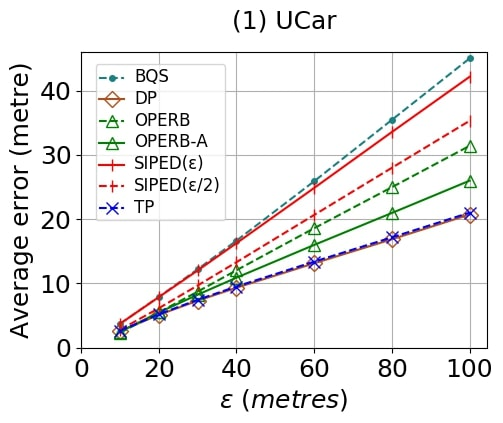
\includegraphics[scale=0.250]{Figures/Exp-PED-error-epsilon-service.jpg}	\hspace{0.5ex}
	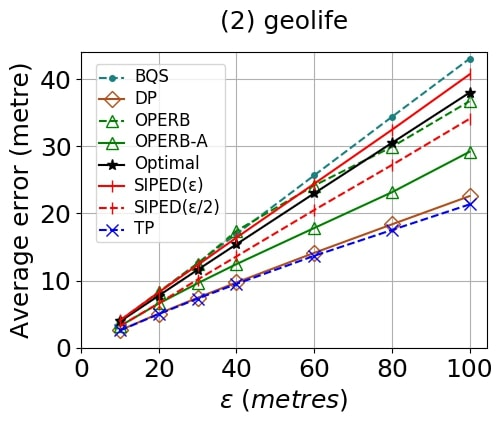
\includegraphics[scale=0.250]{Figures/Exp-PED-error-epsilon-geolife.jpg}	\hspace{0.5ex}
	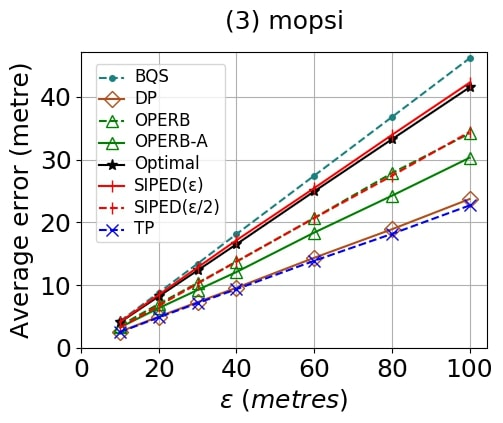
\includegraphics[scale=0.250]{Figures/Exp-PED-error-epsilon-mopsi.jpg}	
	\vspace{-2ex}
	\caption{\small Evaluation of average errors (\ped) on full datasets: varying the error bound $\epsilon$.}
	\label{fig:ae-ped-epsilon}
	\vspace{-2ex}
\end{figure*}
\begin{figure*}[tb!]
	\centering
	%\includegraphics[scale=0.250]{Figures/Exp-SED-error-epsilon-taxi.jpg} \hspace{0.5ex}
	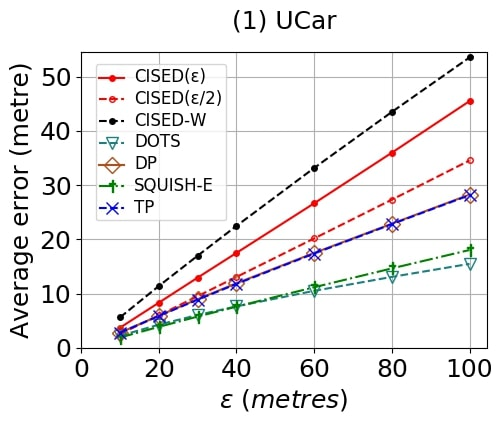
\includegraphics[scale=0.250]{Figures/Exp-SED-error-epsilon-service.jpg}	\hspace{0.5ex}
	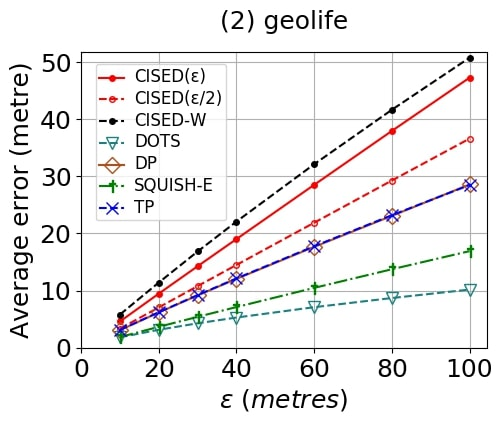
\includegraphics[scale=0.250]{Figures/Exp-SED-error-epsilon-geolife.jpg}	\hspace{0.5ex}
	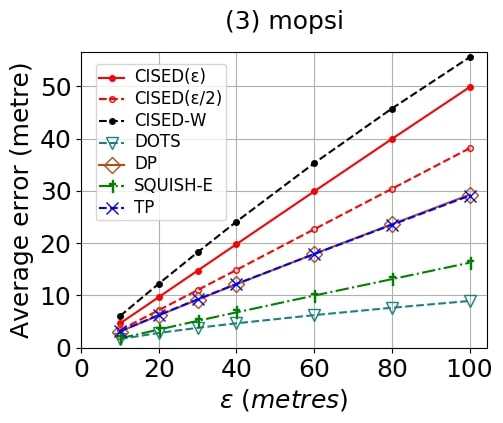
\includegraphics[scale=0.250]{Figures/Exp-SED-error-epsilon-mopsi.jpg}		
	\vspace{-2ex}
	\caption{\small Evaluation of average errors (\sed) on full datasets: varying the error bound $\epsilon$.}
	\label{fig:ae-sed-epsilon}
	\vspace{-2ex}
\end{figure*}
\begin{figure*}[tb!]
	\centering
	%\includegraphics[scale=0.250]{Figures/Exp-DAD-error-epsilon-taxi.jpg} \hspace{0.5ex}
	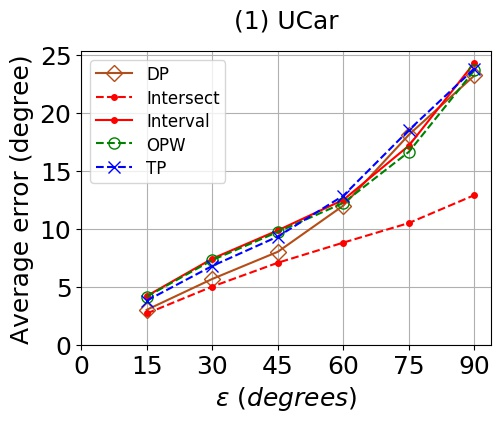
\includegraphics[scale=0.348]{Figures/Exp-DAD-error-epsilon-service.jpg}	\hspace{0.5ex}
	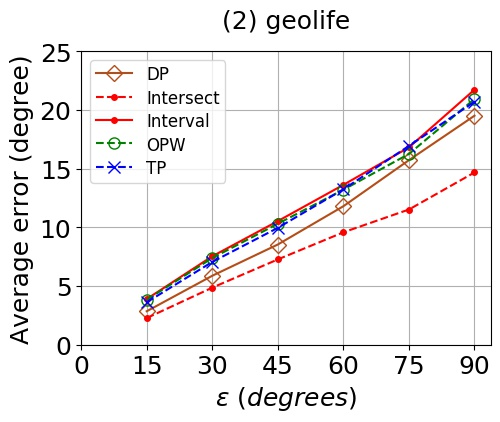
\includegraphics[scale=0.348]{Figures/Exp-DAD-error-epsilon-geolife.jpg}	\hspace{0.5ex}
	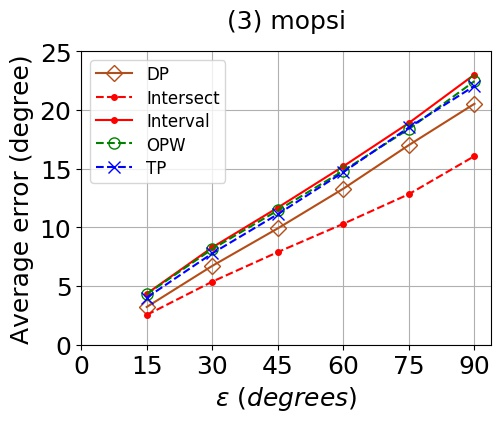
\includegraphics[scale=0.3480]{Figures/Exp-DAD-error-epsilon-mopsi.jpg}	
	\vspace{-2ex}
	\caption{\small Evaluation of average errors (\dad) on full datasets: varying the error bound $\epsilon$.}
	\label{fig:ae-dad-epsilon}
	\vspace{-2ex}
\end{figure*}





\sstab (3) When using \sed, the average errors from the smallest
to the largest are online algorithm {\dagots}, online algorithm \squishe, batch algorithms \tpa and \dpa,
one-pass algorithm \cised($\frac{\epsilon}{2}$),  the \opt algorithm and one-pass algorithm \cised(${\epsilon}$), and one-pass algorithm {\cised-W}.
%
Algorithms \tpa and \dpa are comparable, and they are on average
{($60.36\%$, $66.11\%$, $62.43\%$) and ($62.54\%$, $67.04\%$, $68.64\%$)} of \opt on datasets \dSets, respectively.
Algorithms {\cised-W}, \cised(${\epsilon}$), \cised($\frac{\epsilon}{2}$), \squishe and {\dagots} are on average {{$(115.24\%, 120.34\%, 123.40\%)$}, ($97.32\%$, $106.74\%$, $108.16\%$), ($75.29\%$, $76.03\%$, $81.44\%$), ($40.61\%$, $38.15\%$, $34.22\%$) and {$(39.12\%, 28.80\%, 23.90\%)$} of \opt on datasets \dSets, respectively.
%
For example, the average errors of algorithms
(\opt, \tpa, \dpa, \squishe, {\dagots}, \cised(${\epsilon}$), \cised($\frac{\epsilon}{2}$),  {\cised-W}) in full \mopsi are ($19.39$, $12.17$, $12.20$,  $6.76$, {$4.67$}, $20.68$, $14.71$,  {$24.12$}) metres, respectively, when $\epsilon$ = $40m$.
%


\sstab {(4) When using \dad, the average errors from the smallest
to the largest are one-pass algorithm \intersec, batch algorithms \dpa and \tpa, one-pass algorithm \interval and online algorithm \opwa, and the optimal algorithm \opt.
\eat{%%%%%%%%%%%%%
For example, in Figure~\ref{fig:ae-dad-ped-epsilon}, in \mopsi, the average errors of algorithms
(\tpa, \dpa, \interval) in terms of \ped are ($65.6$, $75.4$, $68.1$) meters, respectively, when $\epsilon$ = $45$ degrees.
It is also worth pointing out that the max errors of algorithms
(\tpa, \dpa, \interval) using \dad may be very large in terms of \ped, \eg they are ($68247.9$, $66794.4$, $68247.9$) meters, respectively, when $\epsilon$ = $45$ degrees.}
}%%%%%%%%%%%%%
Algorithms \tpa, \opwa and \interval are comparable, and they are on average
{($91.35\%$, $61.45\%$, $73.71\%$), ($91.95\%$, $61.37\%$, $76.17\%$) and ($90.36\%$, $68.23\%$, $163.47\%$)} of \opt on datasets \dSets, respectively.
Algorithms \intersec and \dpa are on average ($62.03\%$, $76.54\%$, $110.69\%$) and ($82.45\%$, $96.52\%$, $137.95\%$) of \opt on datasets \dSets, respectively.

\begin{figure*}[tb!]
	\centering
	%\includegraphics[scale=0.250]{Figures/Exp-PED-error-size-taxi.jpg}\hspace{0.5ex}
	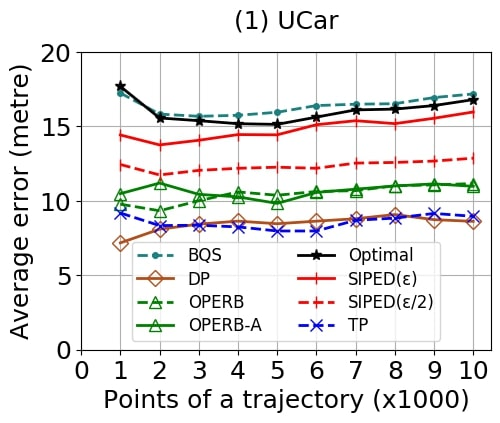
\includegraphics[scale=0.250]{Figures/Exp-PED-error-size-service.jpg} 	\hspace{0.5ex}
	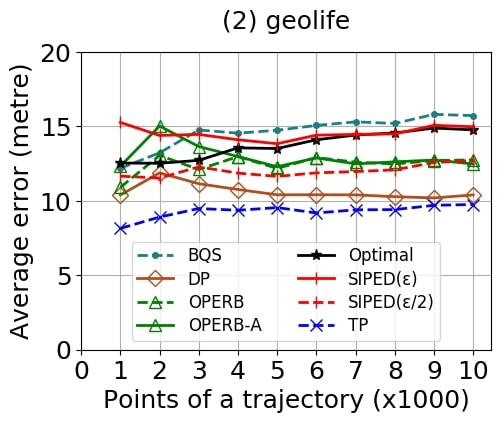
\includegraphics[scale=0.250]{Figures/Exp-PED-error-size-geolife.jpg}	\hspace{0.5ex}
	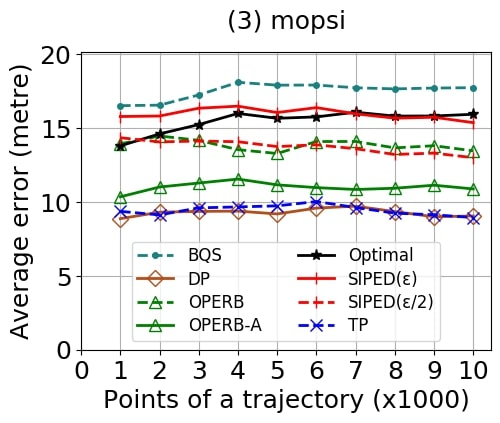
\includegraphics[scale=0.250]{Figures/Exp-PED-error-size-mopsi.jpg}		
	\vspace{-2ex}
	\caption{\small Evaluation of average errors (\ped) on small datasets: varying the size of
		trajectories.}
	\label{fig:ae-ped-size}
	\vspace{-2ex}
\end{figure*}
\begin{figure*}[tb!]
	\centering
	%\includegraphics[scale=0.250]{Figures/Exp-SED-error-size-taxi.jpg}\hspace{0.5ex}
	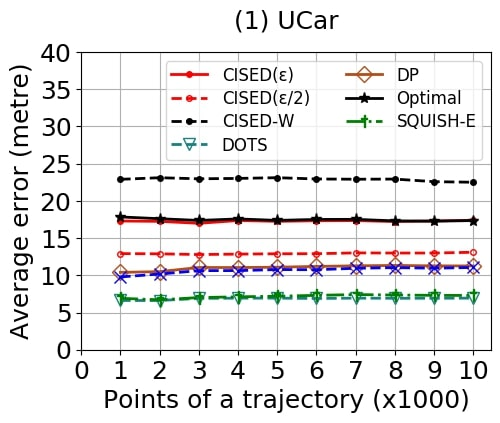
\includegraphics[scale=0.250]{Figures/Exp-SED-error-size-service.jpg} 	\hspace{0.5ex}
	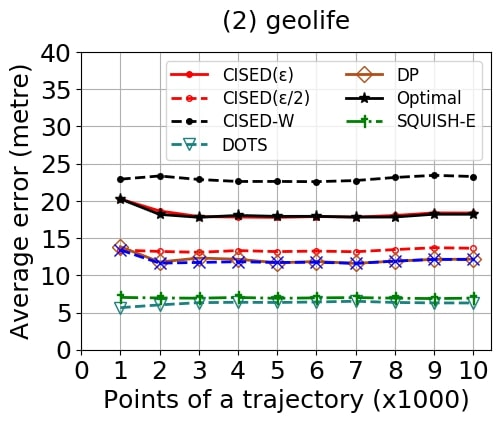
\includegraphics[scale=0.250]{Figures/Exp-SED-error-size-geolife.jpg}	\hspace{0.5ex}
	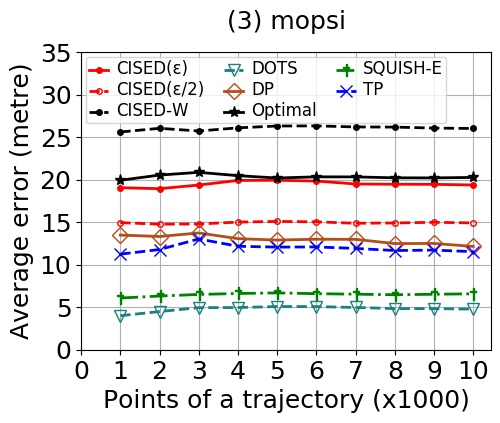
\includegraphics[scale=0.348]{Figures/Exp-SED-error-size-mopsi.jpg}		
	\vspace{-2ex}
	\caption{\small Evaluation of average errors (\sed) on small datasets: varying the size of
		trajectories.}
	\label{fig:ae-sed-size}
	\vspace{-2ex}
\end{figure*}
\begin{figure*}[tb!]
	\centering
	%\includegraphics[scale=0.50]{Figures/Exp-DAD-error-size-taxi.jpg} \hspace{0.5ex}
	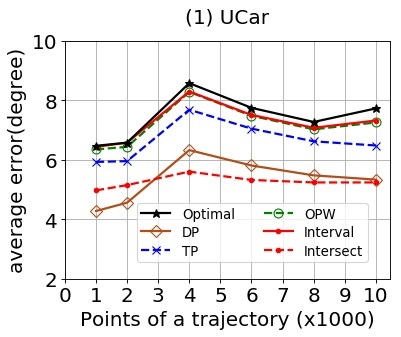
\includegraphics[scale=0.52]{Figures/Exp-DAD-error-size-service.jpg}	\hspace{0.5ex}
	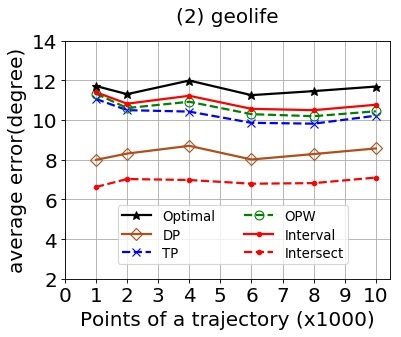
\includegraphics[scale=0.52]{Figures/Exp-DAD-error-size-geolife.jpg}	\hspace{0.5ex}
	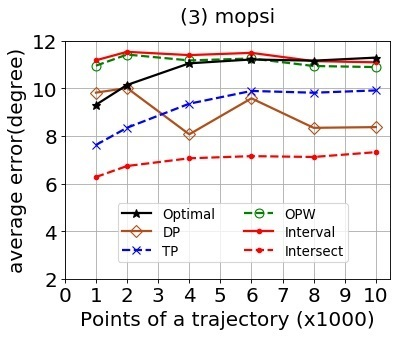
\includegraphics[scale=0.52]{Figures/Exp-DAD-error-size-mopsi.jpg}	
	\vspace{-2ex}
	\caption{\small Evaluation of average errors (\dad) on small datasets: varying the size of trajectories.}
	\label{fig:ae-dad-size}
	\vspace{-2ex}
\end{figure*}


We then present analyses from the views of \lsa algorithms and distance metrics.


\stitle{Analyses of \lsa algorithms}. The average errors of these algorithms  are generally on the contrary of compression ratios. The optimal algorithm is usually  the worst algorithm in terms of average errors, followed by one-pass algorithms and then batch algorithms.
Online algorithms have varied average errors, ranging from the best to the worst.
(1) For batch algorithms, both bottom-up algorithm (\tpa) and top-down algorithm (\dpa) have similar average errors, and they are pretty good compared with other algorithms.
%
(2) Online algorithms \bqsa and \opwa often have the largest average errors in all sub-optimal algorithms, while {\dagots}~and \squishe have the smallest. This is also on the contrary of their compression ratios.
%
(3) For one-pass algorithms, the full $\epsilon$ sector/cone/range combining with a position/direction constraint always have larger average errors than the half $\epsilon$ sector/cone/range.
%
Local distance checking approaches try to include more points into a line segment, this greedy strategy is likely leading to larger average errors, considerably larger than batch algorithms that have the similar compression ratios as one-pass and online algorithms.


\stitle{Analyses of distance metrics}.
For the same error bound $\epsilon$, the average errors of algorithms using \sed are a bit larger than using \ped. {As we know that \ped error is originally caused by the direction changes of a moving object while \sed error is caused by the changes of both the direction and the speed of a moving object, the above phenomenon probably reveals that the changes of speeds are more frequent than the changes of directions for moving objects.}
%
In practice (\eg $\epsilon = 60$ meters and $\epsilon = 45$ degrees), the average errors of algorithms using \dad, when translated to position errors like \ped, are likely $10$ times larger than algorithms directly using \ped and \sed. This is obvious as a small direction deviation with a long trip may lead to a large position error.




\eat{
\sstab (1) When increasing $\epsilon$, the average errors increase linearly.

\sstab (2) Datasets have few impacts on the average errors.

\sstab (1) Trajectory sizes have few impacts on average errors.

\sstab (2) The average errors in this test are consistent with test Exp-2.1.
}






%%%%%%%%%%%%%%%%%%%%%%%%%%%%%%%%%%%%%%%%%%%%%%%%%%%%%%%%%%%%%%%%%%%%%%%%%%%%%%
%\vspace{-1ex}
\subsubsection{Evaluation and \myblue{Analysis} of Efficiency}
%%%%%%%%%%%%%%%%%%%%%%%%%%%%%%%%%%%%%%%%%%%%%%%%%%%%%%%%%%%%%%%%%%%%%%%%%%%%%%

In this set of tests, we compare the efficiency of these algorithms.
The results are reported in Figures~\ref{fig:time-epsilon-ped},~\ref{fig:time-epsilon-sed},~\ref{fig:time-epsilon-dad},~\ref{fig:time-size-ped},~\ref{fig:time-size-sed} and~\ref{fig:time-size-dad}.
Note that even on the small datasets, \emph{the running time of algorithm \opt  is thousands of times slower than one-pass algorithms}. As it is not clear to show all these algorithms in a single figure, only the results of sub-optimal algorithms are shown in these figures.
We first report our findings.



\sstab (1) {Datasets do not have obvious impacts on the running time of \lsa algorithms except \dagots. }

	
\sstab (2) When using \ped, in most cases, the running time from the smallest to the largest is one-pass algorithms \siped, \operb and {\operb-A}, batch algorithms \tpa and \dpa, and online algorithm \bqsa.
Algorithms \siped($\frac{\epsilon}{2}$), {\operb} and {\operb-A} are comparable, algorithm \siped(${\epsilon}$) is $(0.92, 0.92, 0.91)$ times of \siped($\frac{\epsilon}{2}$), and algorithms \tpa, \dpa and \bqsa are on average
($26.79$, $28.25$, $29.87$), ($16.32$, $15.40$, $11.02$) and ($37.73$, $62.23$, $61.29$)
times slower than one-pass algorithm \siped($\frac{\epsilon}{2}$) on datasets \dSets, respectively.
For example, in \mopsi, the running time of algorithms
(\tpa, \dpa, \bqsa, \siped(${\epsilon}$), \siped($\frac{\epsilon}{2}$), \operb, {\operb-A} ) is ($232.9$, $124.2$, $469.4$, $6.89$, $7.6$, $8.6$, {$9.4$}) seconds when $\epsilon$ = $40m$.



\begin{figure*}[tb!]
	\centering
	%\includegraphics[scale=0.250]{Figures/Exp-PED-time-epsilon-taxi.jpg}	\hspace{0.5ex}
	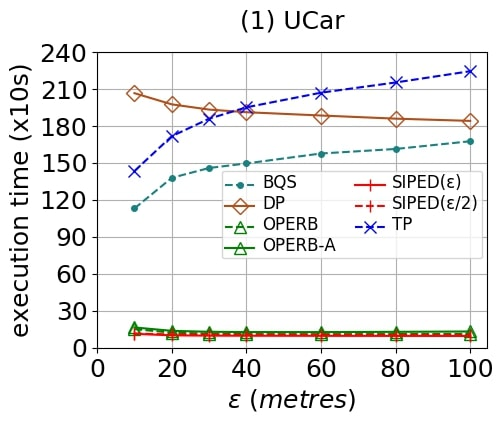
\includegraphics[scale=0.250]{Figures/Exp-PED-time-epsilon-service.jpg}	\hspace{0.5ex}
	\includegraphics[scale=0.250]{Figures/Exp-PED-time-epsilon-geolife.jpg}	\hspace{0.5ex}
	\includegraphics[scale=0.250]{Figures/Exp-PED-time-epsilon-mopsi.jpg}	
	\vspace{-2ex}
	\caption{\small Evaluation of running time (\ped) on full datasets: varying the error bound $\epsilon$.}\label{fig:time-epsilon-ped}
	\vspace{-2ex}
\end{figure*}

\begin{figure*}[tb!]
	\centering
	%\includegraphics[scale=0.250]{Figures/Exp-SED-time-epsilon-taxi.jpg}	\hspace{0.5ex}
	\includegraphics[scale=0.250]{Figures/Exp-SED-time-epsilon-service.jpg}	\hspace{0.5ex}
	\includegraphics[scale=0.250]{Figures/Exp-SED-time-epsilon-geolife.jpg}	\hspace{0.5ex}
	\includegraphics[scale=0.250]{Figures/Exp-SED-time-epsilon-mopsi.jpg}	
	\vspace{-2ex}
	\caption{\small Evaluation of running time (\sed) on full datasets: varying the error bound $\epsilon$.}\label{fig:time-epsilon-sed}
	\vspace{-2ex}
\end{figure*}

\begin{figure*}[tb!]
	\centering
	%\includegraphics[scale=0.250]{Figures/Exp-DAD-time-epsilon-taxi.jpg}\hspace{0.5ex}
	\includegraphics[scale=0.250]{Figures/Exp-DAD-time-epsilon-service.jpg} 	\hspace{0.5ex}
	\includegraphics[scale=0.250]{Figures/Exp-DAD-time-epsilon-geolife.jpg}	\hspace{0.5ex}
	\includegraphics[scale=0.250]{Figures/Exp-DAD-time-epsilon-mopsi.jpg}		
	\vspace{-2ex}
	\caption{\small Evaluation of running time (\dad) on full datasets: varying the error bound $\epsilon$.}\label{fig:time-epsilon-dad}
	\vspace{-2ex}
\end{figure*}



\sstab (3) When using \sed, the running time of algorithms except \dagots~from the smallest to the largest is one-pass algorithms \cised and {\cised-W}, online algorithm \squishe, and batch algorithms \tpa and \dpa, while \dagots~has varied running time. In full datasets, \dagots~runs faster than, comparable with and slower than \dpa in datasets \ucar, \geolife and \mopsi, respectively, while in small datasets, it often runs faster than \dpa.
Algorithm \cised(${\epsilon}$) is $(1.17, 1.17, 0.91)$ times of \cised($\frac{\epsilon}{2}$), and algorithms \tpa, \dpa and \squishe are on average
 ($13.33$, $15.81$, $13.09$), ($12.93$, $10.64$, $8.79$) and
($2.75$, $2.78$, $2.57$) times slower than \cised($\frac{\epsilon}{2}$) on datasets \dSets, respectively.
%
For example, in \mopsi, the running time of algorithms
(\tpa, \dpa, {\dagots}, \squishe, \cised($\epsilon$), \cised($\frac{\epsilon}{2}$), {\cised-W}) is ($156.6$, $104.8$, {$361.1$}, $27.2$, $11.6$, $9.7$, {$9.7$}) seconds when $\epsilon$ = $40m$.

\sstab {(4) When using \dad,} {one-pass algorithms \intersec and \interval run much faster than batch algorithms \tpa and \dpa and online algorithm \opwa.}
%
%Algorithm \interval is a bit slower than \intersec, and algorithms \tpa and \dpa are on average
%($6.66$, $13.55$, $12.73$, $12.73$) and ($11.67$, $14.24$, $16.51$, $17.59$)
%times slower than \interval on datasets \dSets, respectively.
%
Algorithm \interval is $(1.80, 1.84, 1.81)$ times slower than \intersec, and algorithms \tpa, \dpa and \opwa are on average
($24.63$, $23.53$, $23.23$), ($25.49$, $30.11$, $31.72$) and ($39.29$, $147.85$, $80.09$)
times slower than \intersec on datasets \dSets, respectively.
%
For example, the running time of algorithms
(\tpa, \dpa, \opwa, \interval, \intersec) is ($105.57$, $152.53$, $240.40$, $8.57$, $4.69$) seconds in \mopsi when
$\epsilon=45$ degrees, respectively.



\begin{figure*}[tb!]
	\centering
	%\includegraphics[scale=0.250]{Figures/Exp-PED-time-size-taxi.jpg}\hspace{0.5ex}
	\includegraphics[scale=0.250]{Figures/Exp-PED-time-size-service.jpg}	\hspace{0.5ex}
	\includegraphics[scale=0.250]{Figures/Exp-PED-time-size-geolife.jpg}	\hspace{0.5ex}
	\includegraphics[scale=0.250]{Figures/Exp-PED-time-size-mopsi.jpg}	
	\vspace{-2ex}
	\caption{\small Evaluation of running time (\ped) on small datasets: varying the size of trajectories.}\label{fig:time-size-ped}
	\vspace{-2ex}
\end{figure*}

\begin{figure*}[tb!]
	\centering
	%\includegraphics[scale=0.250]{Figures/Exp-SED-time-size-taxi.jpg}\hspace{0.5ex}
	\includegraphics[scale=0.250]{Figures/Exp-SED-time-size-service.jpg}	\hspace{0.5ex}
	\includegraphics[scale=0.250]{Figures/Exp-SED-time-size-geolife.jpg}	\hspace{0.5ex}
	\includegraphics[scale=0.348]{Figures/Exp-SED-time-size-mopsi.jpg}	
	\vspace{-2ex}
	\caption{\small Evaluation of running time (\sed) on small datasets: varying the size of trajectories.}\label{fig:time-size-sed}
	\vspace{-2ex}
\end{figure*}

\begin{figure*}[tb!]
	\centering
	%\includegraphics[scale=0.50]{Figures/Exp-DAD-time-size-taxi.jpg}\hspace{0.5ex}
	\includegraphics[scale=0.52]{Figures/Exp-DAD-time-size-service.jpg} 	\hspace{0.5ex}
	\includegraphics[scale=0.52]{Figures/Exp-DAD-time-size-geolife.jpg}	\hspace{0.5ex}
	\includegraphics[scale=0.52]{Figures/Exp-DAD-time-size-mopsi.jpg}		
	\vspace{-2ex}
	\caption{\small Evaluation of running time (\dad) on small datasets: varying the size of trajectories.}\label{fig:time-size-dad}
	\vspace{-2ex}
\end{figure*}


%\sstab (2) When using \ped, the running time from the smallest to the largest are one-pass algorithms \siped and \operb, and batch and online algorithms \tpa, \dpa and \bqsa. Algorithms \siped and \operb are comparable. Algorithms \tpa, \dpa and \bqsa are comparable, and they are on average \textcolor{red}{($3.8$--$5.3$, $3.5$--$4.8$, $4.6$--$7.2$, $6.2$--$8.4$)} times slower than the one-pass algorithms \siped and \operb on datasets \dSets, respectively.

%\sstab (3) When using \sed, the running time from the smallest to the largest are one-pass algorithm \cised, online algorithm \squishe, and batch algorithms \tpa and \dpa.  Algorithms \squishe, \tpa and \dpa are on average \textcolor{red}{($9.6$--$17.6$, $8.8$--$15.4$, $8.4$--$16.3$, $9.0$--$14.4$)}, \textcolor{red}{($9.6$--$17.6$, $8.8$--$15.4$, $8.4$--$16.3$, $9.0$--$14.4$)} and \textcolor{red}{($9.6$--$17.6$, $8.8$--$15.4$, $8.4$--$16.3$, $9.0$--$14.4$)} times slower than \cised on datasets \dSets, respectively.

%\sstab (4) Batch algorithms \dpa and \tpa using \sed run a bit faster than using \ped, while the one-pass algorithm \cised run \textcolor{red}{$2.0$--$3.0$} times slower than \siped and \operb.


We then present analyses from the views of \lsa algorithms and distance metrics.





\stitle{Analyses of \lsa algorithms.}
The running time from the fastest to the slowest is one-pass algorithms, online and batch algorithms, and optimal algorithms.

For batch algorithms, the running time of \dpa and \tpa decreases or increases with the increase of error bound $\epsilon$, respectively, due to the top-down and bottom-up approaches that they apply. When using \ped or \sed, top-down algorithm usually runs faster than bottom-up algorithm when the error bound $\epsilon$~is large (\eg in \geolife, $\epsilon >10$ metres when using \ped and $\epsilon >30$ metres when using \sed), which means that top-down (bottom-up) algorithm needs to split (merge) the original trajectory fewer (more) times in these cases, vice versa. When using \dad,  top-down algorithms are normally a bit slower than bottom-up algorithms (recall that top-down algorithms have poorer compression ratios compared with bottom-up algorithms, which means that it needs more time to split the raw trajectory into more sub-trajectories).
In addition to error bounds, sampling rates also have impacts on the efficiency of batch algorithms. A dataset with high sampling rate likely needs more merging processes than splitting processes, thus, top-down algorithms run faster than bottom-up algorithms in high sampling datasets when using \ped or \sed.

For online algorithms, \squishe is faster than \bqsa and \opwa at a cost of poorer compression ratios, and it is still a few times slower than one-pass algorithms. \bqsa and \opwa both have poor efficiency as they finally need batch approaches to simplify buffered data, and batch approaches running in a buffer are still time consuming. {\dagots~runs very slow on the full datasets, partially because its frequent copying of memory wastes a lot of time and becomes its bottleneck of efficiency.}

For one-pass algorithms, \operb, \siped, \cised and \interval show a linear running time that is consistent with their time complexity analyses. They are not very sensitive to error bound $\epsilon$, and also scale well with the increase of trajectory size on all datasets as a data point is processed only one time during the whole process.
Algorithms \siped, \operb and \interval have similar running time, and algorithm \cised runs a bit slower than them, partially because finding the common intersection of spatial-temporal cones is a heavier work than sectors or ranges.

{As we analyzed above, different algorithms show different trends with error bounds because they adopt different routines and principles for trajectory compression.}
{Further, weak simplification algorithms have similar running time to their corresponding strong simplification algorithms as they share the same key routines for trajectory compression.}



\stitle{Analyses of distance metrics.}
The computation time of \dad is faster than \ped and \sed, and the computation time of \ped and \sed are 2.3 and 1.7 times of \dad, respectively.
{It is also worth pointing out that algorithms \dpa using \ped, \sed and \dad have similar running time in all datasets, though the computation of \ped is much heavier than \sed and \dad. The reason is that \dpa using \ped has the best compression ratios which instead leads to the least splitting processes in the top-down manner. Combining these two factors, \ie the computing of distance/direction deviation and the processing of trajectory splitting, finally, algorithm \dpa using \ped has similar running time as \dpa using \dad or \sed.}

%%%%%%%%%%%%%%%%%%%%%%%%%%%%%%%%%%%%%%%%%%%%%%%%%%%%%%%%%%%%%%%%%%%%%%%%%%%%%%
\subsubsection{{Evaluation and \myblue{Analysis} of Data Aging}}
%%%%%%%%%%%%%%%%%%%%%%%%%%%%%%%%%%%%%%%%%%%%%%%%%%%%%%%%%%%%%%%%%%%%%%%%%%%%%%
\label{sec:exp-data-aging}
In this set of tests, we compare the errors and compression ratios of algorithms in data aging. We set $\epsilon_1=40m$ (or $\epsilon_1=30^o$) in the first run and $\epsilon_2=60m$ (or $\epsilon_2=50^o$) in the second run. Besides, we also run these algorithms on the raw trajectories, setting $\epsilon_3=\epsilon_1 + \epsilon_2=100m$ (or $\epsilon_3=80^o$). The max errors are reported in \mytable{tab:aging-me}, and the compression ratios are reported in \mytable{tab:aging-cr} and \mytable{tab:cr}, respectively.

\ni (1) Algorithms \dpa using \ped and \sed both have max errors less than $\epsilon_2 = 60m$, confirming that they are aging friendly and their max errors are consistent with Theorem ~\ref{theo-aging-error-dp}; while algorithm \dpa using \dad and other algorithms have max error larger than $\epsilon_2 = 60m$ or $\epsilon_2 = 50^o$, confirming that they are not aging friendly and their max errors are consistent with Theorems ~\ref{theo-aging-dp-dad}, \ref{theo-aging-tp} and \ref{theo-aging-online}.

\ni (2) Algorithm \dpa using \dad and other algorithms have max error less than $\epsilon_1 + \epsilon_2 = 100m$ or $\epsilon_1 + \epsilon_2 = 80^o$, which is consistent with Theorem ~\ref{theo-aging-distance}.

\ni (3) \mytable{tab:aging-cr} and \mytable{tab:cr} tell that, if algorithms compress data using $\epsilon_1$ and $\epsilon_2$ in turn, then they have a bit poorer compression ratios than directly using $\epsilon_3=\epsilon_1 + \epsilon_2$.
Note that the causes of this phenomenon are varied. For algorithm \dpa using \ped or \sed, it is caused by the shorten of the final error bound, which is $max\{\epsilon_1, \epsilon_2\}$, less than $\epsilon_3=\epsilon_1 + \epsilon_2$; while for the other algorithms, they lose some compression ratios because of data aging.


\begin{table}
	%\renewcommand{\arraystretch}{1.2}
	\caption{\small The max errors of algorithms in data aging that set $\epsilon_1=40m$ (or $\epsilon_1=30^o$ when using \dad) in the first run and $\epsilon_2=60m$ (or $\epsilon_2=50^o$ when using \dad) in the second run.}
	\centering
	\scriptsize
	\vspace{-1ex}
	\begin{tabular}{|l|c|c|c|l|c|c|c|l|c|c|c|}
		\hline
		\bf{Alg. (PED)}  &\ucar &\geolife &\mopsi & \bf{Alg. (SED)}  &\ucar &\geolife &\mopsi &\bf{Alg. (DAD)}  &\ucar &\geolife &\mopsi \\
		\hline
		{\dpa} &	$59.99$ & $59.99 $ &	$59.99$	&\dpa &$59.99$ &$59.99$ & $59.99$ & \dpa	& $79.90$	& $79.93$	& $78.96 $ \\
		\hline
		{\tpa} &	$99.56$ & $96.95$ &	$93.00$	&\tpa 	& $97.55$& $96.70$ &$90.53$ & \tpa	& $79.94$	& $79.93$	& $79.64$ \\
		\hline
		{\bqsa} &	$96.20 $ & $93.58  $ &	$96.79 $	&\squishe &$92.60$ &$90.89$ & $84.38$ & \opwa	& $79.96$	& $79.96$	& $79.74$ \\
		\hline
		{\siped($\epsilon$)} &	$97.34   $ & $95.21  $ &	$98.86   $	&\cised($\epsilon$) & $97.75$ &$97.51$ &$96.65$ & \interval	& $79.96$	& $79.93$	& $79.74$ \\
		\hline
		{\siped($\frac{\epsilon}{2}$)} &	$99.18  $ & $94.57  $ &	$97.91  $ &\cised($\frac{\epsilon}{2}$) &$ 97.40 $ & $97.51$ & $98.83$& \intersec	& $70.26 $	& $77.78$	& $72.87$ \\
		\hline
		{\operb} &	${98.26} $ & ${96.53} $ & ${98.08} $	& {\dagots} &98.47 &95.92 &96.7 & / &- &- &- \\
		\hline
		{\operb-A} &	${99.99} $ & ${99.99} $ & ${99.99} $	& {\cised-W} &99.21 &99.34 &98.81 & / &- &- &- \\
		\hline
	\end{tabular}
	\label{tab:aging-me}

	\vspace{-1ex}
\end{table}


   	 	
\begin{table}
	%\renewcommand{\arraystretch}{1.2}
	\caption{\small The final compression ratios of algorithms in data aging that set $\epsilon_1=40m$ (or $\epsilon_1=30^o$ when using \dad) in the first run and $\epsilon_2=60m$ (or $\epsilon_2=50^o$ when using \dad) in the second run.}
	\centering
	\scriptsize
	%\vspace{-1ex}
	\begin{tabular}{|l|c|c|c|l|c|c|c|l|c|c|c|}
		\hline
		\bf{Alg. (PED)}  &\ucar &\geolife &\mopsi & \bf{Alg. (SED)}  &\ucar &\geolife &\mopsi &\bf{Alg. (DAD)}  &\ucar &\geolife &\mopsi \\
		\hline  		
		{\dpa} &	$4.67$ & $1.94 $ &	$1.68$	&\dpa &$10.03$ &$3.83$ & $2.78 $ & \dpa	& $12.75$	& $22.20$	& $20.34 $ \\
		\hline
		{\tpa} &	$4.66$ & $	2.07 $ &	$1.74 $	&\tpa 	& $10.09$& $3.78$ &$2.76$ & \tpa	& $3.80$	& $13.28$	& $11.30$ \\
		\hline
		{\bqsa} &	$4.13$ & $1.67 $ &	$ 1.43 $	&\squishe &$11.38$ &$4.55$ & $3.47$ & \opwa	& $4.09$	& $13.88$	& $11.92$ \\
		\hline
		{\siped($\epsilon$)} &	$4.15 $ & $1.69 $ &	$1.42$	&\cised($\epsilon$) & $9.12$ &$3.28$ &$2.45 $ & \interval	& $3.81$	& $13.37$	& $11.47 $ \\
		\hline
		{\siped($\frac{\epsilon}{2}$)} &	$4.65 $ & $1.94$ &	$1.68$ &\cised($\frac{\epsilon}{2}$) &$10.66 $ & $3.94$ & $2.99 $& \intersec	& $5.37$	& $17.11$	& $15.05 $ \\
		\hline
		{\operb} &	$5.03$ & $2.03 $ &	$ 1.97 $	& {\dagots} &11.81 &3.89 &2.55 & / &- &- & - \\
		\hline
		{\operb-A} &	${5.53} $ & ${1.90} $ & ${1.93} $	& {\cised-W} &8.94 &3.76 &2.34 & / &- &- &- \\
		\hline
	\end{tabular}
	\label{tab:aging-cr}	
	\vspace{-1ex}
\end{table}
  	 	
\begin{table}
	%\renewcommand{\arraystretch}{1.2}
	\caption{\small The compression ratios of algorithms running on the raw trajectories that set $\epsilon_3=\epsilon_1+\epsilon_2=100m$ (or $\epsilon_3=80^o$ when using \dad).}
	\centering
	\scriptsize
	%\vspace{-1ex}
	\begin{tabular}{|l|c|c|c|l|c|c|c|l|c|c|c|}
		\hline
		\bf{Alg. (PED)}  &\ucar &\geolife &\mopsi & \bf{Alg. (SED)}  &\ucar &\geolife &\mopsi &\bf{Alg. (DAD)}  &\ucar &\geolife &\mopsi \\
		\hline
		{\dpa} &	$3.64$ & $ 1.17$ &	$1.39$	&\dpa &$7.44$ & $2.69$ &$1.91$  & \dpa	& $8.25$	& $15.17$	& $17.04$ \\
		\hline
		{\tpa} &	$3.70 $ & $1.22$ &	$1.50 $	&\tpa 	& $7.56 $& $2.70$ & $1.73 $ & \tpa	& $2.47 $	& $ 	7.51 $	& $ 	9.42  $ \\
		\hline
		{\bqsa} &	$3.23$ & $1.71$ &	$1.39 $	&\squishe &$10.36 $ & $4.10  $ & $2.82$ & \opwa	& $3.23$	& $8.66$	& $10.75$ \\
		\hline
		{\siped($\epsilon$)} &	$3.25$ & $ 1.04$ &	$1.28 $	&\cised($\epsilon$) & $6.68 $ &$ 2.35$ &$ 1.49	$ & \interval	& $2.79 $	& $8.01$	& $9.95 $ \\
		\hline
		{\siped($\frac{\epsilon}{2}$)} &	$3.81 $ & $1.29 $ &	$1.55 $ &\cised($\frac{\epsilon}{2}$) &$8.02  $ & $2.90$ & $1.87$& \intersec	& $4.32 $	& $11.75$	& $13.61 $ \\
		\hline
		{\operb} &	$4.08 $ & $1.43 $ & $1.56 $	& {\dagots} &10.91 &4.33 &3.43 & /&- &- &- \\
		\hline
		{\operb-A} &	${4.06} $ & ${1.31} $ & ${1.20} $	& {\cised-W} &6.92 &2.98 &1.77 & / &- &- &- \\
		\hline
	\end{tabular}
	\label{tab:cr}	
	\vspace{-1ex}
\end{table}

\begin{table}
	%\renewcommand{\arraystretch}{1.2}
	\caption{\small The max errors of {\emph{where\_at}} queries on the compressed trajectories: fixed $\epsilon=40m$ or $30^o$ when using \dad.}
	\centering
	\scriptsize
	%\vspace{-1ex}
	\begin{tabular}{|l|c|c|c|l|c|c|c|}
		\hline
		\bf{Alg. (PED)}  &\ucar &\geolife &\mopsi & \bf{Alg. (DAD)}  &\ucar &\geolife &\mopsi \\
		\hline
		{\dpa} &	$3.48 \times 10^6$ & $1.83 \times 10^6$ &	$5.03 \times 10^6$	& \dpa	& $2.76 \times 10^6$	& $7.91 \times 10^5$	& $4.87 \times 10^5$ \\
		\hline
		{\tpa} &	$3.51 \times 10^6$ & $1.91 \times 10^6$ &	$5.03 \times 10^6$	& \tpa	& $2.76 \times 10^6$	& $7.91 \times 10^5$	& $5.01 \times 10^5$ \\
		\hline
		{\bqsa} &	$3.51 \times 10^6$ & $1.94 \times 10^6$ &	$1.40 \times 10^6$	& \opwa	& $2.76 \times 10^6$	& $7.91 \times 10^5$	& $5.01 \times 10^5$ \\
		\hline
		{\siped($\epsilon$)} &	$3.51 \times 10^6$ & $1.02 \times 10^6$ &	$1.39 \times 10^6$	& \interval	& $2.76 \times 10^6$	& $7.91 \times 10^5$	& $5.01 \times 10^5$ \\
		\hline
		{\siped($\epsilon/2$)} &	$3.50 \times 10^6$ & $1.02 \times 10^6$ &	$1.39 \times 10^6$	& \intersec	& $2.76 \times 10^6$	& $7.91 \times 10^5$	& $4.18 \times 10^5$ \\
		\hline
		{\operb} &	$3.50 \times 10^6$ & $1.56 \times 10^6$ &	$1.39 \times 10^6$	& / & -  & - & -  \\
		\hline
		{\operb-A} &	${7.50\times 10^6} $ & ${1.84\times 10^6} $ & ${5.03\times 10^6} $ & / &- &- &- \\
		\hline
	\end{tabular}
	\label{tab:query-me}
	\vspace{0.5ex}
	\\{Note that all algorithms using \sed have the max query errors not more than the error bound, \ie $\epsilon=40m$ here.}
	\vspace{-1ex}
\end{table} 	 	



%In the contrast, algorithms \dpa using \ped and \sed do not loss that. Hence, given the same final error bound (\eg $100m$) of data aging, algorithm \dpa using \ped (or \sed) shows a bit advantages in terms of compression ratios.



\stitle{Analyses of \lsa algorithms.} \dpa is the only algorithm that is aging friendly \wrt ~\ped and \sed, {and all algorithms have bounded errors}. Indeed, {aging friendliness} is a result of the {specific nature} of algorithm \dpa, \ie batch and top-down, that always splits a trajectory into two sub-trajectories by the same splitting point when it uses any \ped or \sed larger than the error bound.

\stitle{Analyses of \lsa distance metrics.} \dad is not aging friendly \wrt to any algorithm. It is different with \ped and \sed in that, the \dad of a point is closely related to its neighbor point while \ped and \sed are not, thus, once its neighbor point is removed, its \dad is also changed. This character makes it not aging friendly \wrt the \dpa algorithm.



 	 	
 	 	


%%%%%%%%%%%%%%%%%%%%%%%%%%%%%%%%%%%%%%%%%%%%%%%%%%%%%%%%%%%%%%%%%%%%%%%%%%%%%%
\subsubsection{{Evaluation and \myblue{Analysis} of Queries Friendliness}}
\label{sec-exp-query}
%%%%%%%%%%%%%%%%%%%%%%%%%%%%%%%%%%%%%%%%%%%%%%%%%%%%%%%%%%%%%%%%%%%%%%%%%%%%%%
We finally evaluate those compressed trajectories from the viewpoint of trajectory application, \ie spatio-temporal query. The well-known spatio-temporal queries are \emph{where\_at, when\_at, range, nearest\_neighbor} and \emph{spatial\_join} \cite{Cao:Spatio,Trajcevski:Uncertainty}. Among them, \emph{where\_at} query, \ie ``\emph{the position $P$ of a moving object at time $t$}'' \cite{Cao:Spatio}, is the foundation of \emph{range} and \emph{nearest\_neighbor} queries, {and \emph{when\_at} query, \ie ``\emph{the time $t$ at which a moving object on a trajectory is expected to be at position $P$}'' \cite{Cao:Spatio}, is also a critical building block for many applications.}
{Hence, we choose them to evaluate compressed trajectories simplified by \lsa algorithms using \ped, \sed and \dad.
As mentioned in \cite{Cao:Spatio,Trajcevski:Uncertainty}, the answer to \emph{where\_at} query is the expected position $P'$ of the moving object at time $t$. Indeed, it is the \emph{synchronized point} of $P$ when the query is performed on simplified trajectories.}

\begin{figure*}[tb!]
	\centering
	\includegraphics[scale = 0.25]{Figures/Exp-where-PED-error-epsilon-service.jpg}\hspace{0.5ex}
	\includegraphics[scale = 0.25]{Figures/Exp-where-PED-error-epsilon-geolife.jpg}\hspace{0.5ex}
	\includegraphics[scale = 0.25]{Figures/Exp-where-PED-error-epsilon-mopsi.jpg}
	\vspace{-2ex}
	\caption{\small Evaluation of {\emph{where\_at}} queries (PED) on full datasets: varying error bound $\epsilon$.}
	\label{fig:query-ped-epsilon}
	\vspace{-1.0ex}
\end{figure*}
\begin{figure*}[tb!]
	\centering
	\includegraphics[scale = 0.250]{Figures/Exp-where-SED-error-epsilon-service.jpg}\hspace{0.5ex}
	\includegraphics[scale = 0.250]{Figures/Exp-where-SED-error-epsilon-geolife.jpg}\hspace{0.5ex}
	\includegraphics[scale = 0.250]{Figures/Exp-where-SED-error-epsilon-mopsi.jpg}
	\vspace{-2ex}
	\caption{\small Evaluation of {\emph{where\_at}} queries (SED) on full datasets: varying error bound $\epsilon$.}
	\label{fig:query-sed-epsilon}
	\vspace{-1.0ex}
\end{figure*}
\begin{figure*}[tb!]
	\centering
	\includegraphics[scale = 0.250]{Figures/Exp-where-DAD-error-epsilon-service.jpg}\hspace{0.5ex}
	\includegraphics[scale = 0.250]{Figures/Exp-where-DAD-error-epsilon-geolife.jpg}\hspace{0.5ex}
	\includegraphics[scale = 0.250]{Figures/Exp-where-DAD-error-epsilon-mopsi.jpg}
	\vspace{-2ex}
	\caption{\small Evaluation of {\emph{where\_at}} queries (DAD) on full datasets: varying error bound $\epsilon$.}
	\label{fig:query-dad-epsilon}
	\vspace{-1.0ex}
\end{figure*}



\stitle{{Exp-1: \emph{where\_at} queries.}}
{We first compress these trajectories using \ped, \sed and \dad, respectively. }
{Then, for each point $P$ in an original trajectory $\dddot{\mathcal{T}}$, we perform a \emph{where\_at} query on each of its compressed trajectories taking time $P.t$ as input, and calculate the distance between the actual position $P$ and the expected position $P'$ to denote the error of queries.
}
%
{The max and average errors of the queries are reported in \mytable{tab:query-me} and Figures~\ref{fig:query-ped-epsilon}, \ref{fig:query-sed-epsilon}, \ref{fig:query-dad-epsilon}, \ref{fig:query-ped-size},\ref{fig:query-sed-size} and \ref{fig:query-dad-size}, respectively.}









\begin{figure*}[tb!]
	\centering
	\includegraphics[scale=0.250]{Figures/Exp-where-PED-error-size-service.jpg} 	\hspace{0.5ex}
	\includegraphics[scale=0.250]{Figures/Exp-where-PED-error-size-geolife.jpg}	\hspace{0.5ex}
	\includegraphics[scale=0.250]{Figures/Exp-where-PED-error-size-mopsi.jpg}		
	\vspace{-2ex}
	\caption{\small Evaluation of {\emph{where\_at}} queries (\ped) on small datasets: varying the size of
		trajectories.}
	\label{fig:query-ped-size}
	\vspace{-1ex}
\end{figure*}

\begin{figure*}[tb!]
	\centering
	\includegraphics[scale=0.250]{Figures/Exp-where-SED-error-size-service.jpg} 	\hspace{0.5ex}
	\includegraphics[scale=0.250]{Figures/Exp-where-SED-error-size-geolife.jpg}	\hspace{0.5ex}
	\includegraphics[scale=0.250]{Figures/Exp-where-SED-error-size-mopsi.jpg}		
	\vspace{-2ex}
	\caption{\small Evaluation of {\emph{where\_at}} queries (\sed) on small datasets: varying the size of
		trajectories.}
	\label{fig:query-sed-size}
	\vspace{-1ex}
\end{figure*}


\begin{figure*}[tb!]
	\centering
	\includegraphics[scale=0.250]{Figures/Exp-where-DAD-error-size-service.jpg}	\hspace{0.5ex}
	\includegraphics[scale=0.250]{Figures/Exp-where-DAD-error-size-geolife.jpg}	\hspace{0.5ex}
	\includegraphics[scale=0.250]{Figures/Exp-where-DAD-error-size-mopsi.jpg}	
	\vspace{-2ex}
	\caption{\small Evaluation of {\emph{where\_at}} queries (\dad) on small datasets: varying the size of trajectories.}
	\label{fig:query-dad-size}
	\vspace{-1ex}
\end{figure*}




\ni (1) When using \ped, the max query errors of all algorithms are more than $10^6$ meters in all datasets, significantly larger than the error bound (40 meters in \mytable{tab:query-me}). The large max errors also lead to larger average query errors, \ie they are greater than error bounds in all datasets.


\ni (2) When using \sed, the max query errors of all algorithms are clear not more than the error bounds, and the average query errors are consistent with those compression errors shown in Section~\ref{sec-ae}.


\ni (3) When using \dad, the max query errors of all algorithms are more than $10^6$ meters in dataset \ucar, and more than $10^5$ meters in datasets \geolife and \mopsi, respectively, also significantly larger than the error bound (40 meters in \mytable{tab:query-me}). Moreover, compared with using \ped, it has few points having query errors larger than error bounds, thus, it has the smallest average query errors in all algorithms and all datasets.



\begin{table}
	%\renewcommand{\arraystretch}{1.2}
	\caption{\small {The max errors {($\times 10^6$ s)} of \emph{when\_at} queries on compressed trajectories: fixed $\epsilon=40m$ or $30^o$ when using \dad.}}
	\centering
	\scriptsize
	\vspace{-1ex}
	\begin{tabular}{|l|c|c|c|l|c|c|c|l|c|c|c|}
		\hline
		\bf{Alg. (PED)}  &\ucar &\geolife &\mopsi & \bf{Alg. (SED)}  &\ucar &\geolife &\mopsi &\bf{Alg. (DAD)}  &\ucar &\geolife &\mopsi \\
		\hline
		{\dpa} &	$11.2$ & $126$ &	$6.59  $	&\dpa &$11.6  $ &$5.01  $ & $1.84 $ & \dpa	& $17.6 $	& $5.88 $	& $3.99 $ \\
		\hline
		{\tpa} &	$26.1$ & $126  $ &	$9.91  $	&\tpa 	& $11.6  $& $5.01  $ &$5.18 $ & \tpa	& $ 17.6 $	& $ 2.90 $	& $ 5.06  $ \\
		\hline
		{\bqsa} &	$11.6$ & $126 $ &	$ 11.5 $	&\squishe &$11.6  $ & $ 18.3  $ & $2.62 $ & \opwa	& $8.19 $	& $ 4.02$	& $5.06 $ \\
		\hline
		{\siped($\epsilon$)} &	$11.5$ & $73.7  $ &	$6.65  $	&\cised($\epsilon$) & $ 11.6 $ &$ 39.7	  $ &$5.48 $ & \interval& $8.19 $	& $4.02 $	& $ 5.06 $ \\
		\hline
		{\siped($\frac{\epsilon}{2}$)} &	$11.5$ & $73.7 $ &	$ 6.68 $ &\cised($\frac{\epsilon}{2}$) &$ 11.6 $ & {$39.7$} & $5.20 $& \intersec	& $ 8.19 $	& $ 2.63 $	& $ 5.06 $ \\
		\hline
		{\operb} &	$21.6 $ & $75.2 $ & $8.31 $	& {\dagots} &$11.6$ &$18.3$ & $2.91$ & /&- &- &- \\
		\hline
		{\operb-A} &	${22.1} $ & ${126} $ & ${11.5} $	&  {\cised-W} &$11.6$ &$47.7$ &$5.50$ & / &- &- &- \\
		\hline
	\end{tabular}
	\label{tab:query-when-me}
	\vspace{-1ex}
\end{table}






\begin{figure*}[tb!]
	\centering
	\includegraphics[scale = 0.350]{Figures/Exp-when-PED-error-epsilon-service.jpg}\hspace{0.5ex}
	\includegraphics[scale = 0.350]{Figures/Exp-when-PED-error-epsilon-geolife.jpg}\hspace{0.5ex}
	\includegraphics[scale = 0.350]{Figures/Exp-when-PED-error-epsilon-mopsi.jpg}
	\vspace{-2ex}
	\caption{\small {Evaluation of \emph{when\_at} queries (PED) on full datasets: varying error bound $\epsilon$.}}
	\label{fig:query-when-ped-epsilon}
	\vspace{-1.0ex}
\end{figure*}
\begin{figure*}[tb!]
	\centering
	\includegraphics[scale = 0.350]{Figures/Exp-when-SED-error-epsilon-service.jpg}\hspace{0.5ex}
	\includegraphics[scale = 0.350]{Figures/Exp-when-SED-error-epsilon-geolife.jpg}\hspace{0.5ex}
	\includegraphics[scale = 0.350]{Figures/Exp-when-SED-error-epsilon-mopsi.jpg}
	\vspace{-2ex}
	\caption{\small {Evaluation of \emph{when\_at} queries (SED) on full datasets: varying error bound $\epsilon$.}}
	\label{fig:query-when-sed-epsilon}
	\vspace{-1.0ex}
\end{figure*}
\begin{figure*}[tb!]
	\centering
	\includegraphics[scale = 0.350]{Figures/Exp-when-DAD-error-epsilon-service.jpg}\hspace{0.5ex}
	\includegraphics[scale = 0.350]{Figures/Exp-when-DAD-error-epsilon-geolife.jpg}\hspace{0.5ex}
	\includegraphics[scale = 0.350]{Figures/Exp-when-DAD-error-epsilon-mopsi.jpg}
	\vspace{-2ex}
	\caption{\small {Evaluation of \emph{when\_at} queries (DAD) on full datasets: varying error bound $\epsilon$.}}
	\label{fig:query-when-dad-epsilon}
	\vspace{-1.0ex}
\end{figure*}

\stitle{{Exp-2: \emph{when\_at} queries.}}
{For each point $P$ in an original trajectory $\dddot{\mathcal{T}}$, we do a \emph{when\_at} query on the simplified trajectory. Since quite a few original data points are not exactly on the line segments of the simplified trajectory, we first map each original point $P$ to its closest point $P'$ having the minimum Euclidean distance on the line segment representing this point along the same way as \cite{Cao:Spatio}, then we get the expected time $P'.t'$ of $P'$ \wrt this line segment in a way inverse to the finding of a synchronized point, and we finally calculate the absolute time difference between the actual time $P.t$ and the expected time $P'.t'$ as the error of the query.}
%
{The max and average errors of the queries are reported in \mytable{tab:query-when-me} and Figures~\ref{fig:query-when-ped-epsilon}, \ref{fig:query-when-sed-epsilon}, \ref{fig:query-when-dad-epsilon}, \ref{fig:query-when-ped-size}, \ref{fig:query-when-sed-size} and \ref{fig:query-when-dad-size}, respectively.}








\begin{figure*}[tb!]
	\centering
	\includegraphics[scale=0.350]{Figures/Exp-when-PED-error-size-service.jpg} 	\hspace{0.5ex}
	\includegraphics[scale=0.350]{Figures/Exp-when-PED-error-size-geolife.jpg}	\hspace{0.5ex}
	\includegraphics[scale=0.350]{Figures/Exp-when-PED-error-size-mopsi.jpg}		
	\vspace{-2ex}
	\caption{\small {Evaluation of \emph{when\_at} queries (\ped) on small datasets: varying the size of
		trajectories.}}
	\label{fig:query-when-ped-size}
	\vspace{-1ex}
\end{figure*}

\begin{figure*}[tb!]
	\centering
	\includegraphics[scale=0.350]{Figures/Exp-when-SED-error-size-service.jpg} 	\hspace{0.5ex}
	\includegraphics[scale=0.350]{Figures/Exp-when-SED-error-size-geolife.jpg}	\hspace{0.5ex}
	\includegraphics[scale=0.350]{Figures/Exp-when-SED-error-size-mopsi.jpg}		
	\vspace{-2ex}
	\caption{\small {Evaluation of \emph{when\_at} queries (\sed) on small datasets: varying the size of
		trajectories.}}
	\label{fig:query-when-sed-size}
	\vspace{-1ex}
\end{figure*}


\begin{figure*}[tb!]
	\centering
	\includegraphics[scale=0.350]{Figures/Exp-when-DAD-error-size-service.jpg}	\hspace{0.5ex}
	\includegraphics[scale=0.350]{Figures/Exp-when-DAD-error-size-geolife.jpg}	\hspace{0.5ex}
	\includegraphics[scale=0.350]{Figures/Exp-when-DAD-error-size-mopsi.jpg}	
	\vspace{-2ex}
	\caption{\small {Evaluation of \emph{when\_at} queries (\dad) on small datasets: varying the size of trajectories.}}
	\label{fig:query-when-dad-size}
	\vspace{-1ex}
\end{figure*}

\ni {(1) The max error of \emph{when\_at} queries on simplified trajectories is unbounded as proved in \cite{Cao:Spatio}. Indeed, the query error is related to the length of the time interval between two neighboring points of a simplified trajectory. We explain this with an example. Suppose that one moves from the front door, quickly passes through the living room, and goes to bed for a long sleep. Since the house is not big, the trajectory is possible simplified to two points, \ie $P_s$ in the front door and $P_e$ on the bed. In this case, a \emph{when\_at} query taking a point $P$ in his living room as input may return the excepted time $t'$ with an error of several hours to the actual time $P.t$.}

\ni {(2) The average error of \emph{when\_at} queries normally increases with the increment of error bounds. This is obvious as the increment of error bounds enlarges the average length of the time interval between two neighboring points in a simplified trajectory, which leads to the increase of the average error of \emph{when\_at} queries. Similarly, the algorithms having better compression ratios typically have larger errors for \emph{when\_at} queries.}
	
\ni {(3) \sed algorithms have smaller average \emph{when\_at} query errors than \ped algorithms, majorly because \sed introduces smaller distance errors and has relatively worse compression ratios compared with \ped. \dad algorithms also have smaller average \emph{when\_at} query errors than \ped algorithms, partially because of their relatively worse  compression ratios compared with \ped. }
	

%%%%%%%%%%%%%%%%%%%%%%%%%%%%%%%%%%%%%%%%%%%%%%%%%%%%%%%%%%%%%%%%%%%%%%%%%%%%%%
%\stitle{Summary}.
\subsubsection{Summary}
\label{sec-exp-summary}
%%%%%%%%%%%%%%%%%%%%%%%%%%%%%%%%%%%%%%%%%%%%%%%%%%%%%%%%%%%%%%%%%%%%%%%%%%%%%%
From these tests we find the followings.

\stitle{\lsa Algorithms}.
\emph{(1)} The optimal algorithms have the best compression ratios, large average errors and the worst efficiencies.
%
\emph{(2)} Batch algorithms, except \dpa using \dad, have good compression ratios, normal average errors and poor efficiency.
%
The bottom-up (\tpa) and top-down (\dpa) algorithms have the similar compression ratios and average errors when using either \ped or \sed. The bottom-up method has obviously better compression ratios than the top-down method when using \dad.
%
The running time of batch algorithms \dpa and \tpa decreases and increases with the increase of error bound $\epsilon$, respectively. When using \ped or \sed, top-down algorithm \dpa usually runs faster than bottom-up algorithm \tpa when the error bound $\epsilon$~is large  (\eg in \geolife, $\epsilon >10$ metres when using \ped and $\epsilon >30$ metres when using \sed). When using \dad, the top-down algorithm is normally a bit slower than the bottom-up algorithm.
Top-down algorithms also run faster than bottom-up algorithms in high sampling datasets when using \ped or \sed.
%
\emph{(3)} Online algorithms \opwa and \bqsa usually have better compression ratios than batch algorithms, the worst average errors, and poorer efficiency than batch algorithms. Algorithm \squishe is on the other side of \opwa and \bqsa,
{and algorithm \dagots~has poor compression ratios, the best average errors and varied efficiency. In our tests (in Java), when \dagots~is processing a long trajectory, the frequent copying of memory makes it even slower than batch algorithms.}
%
\emph{(4)} One-pass algorithms \operb, \siped, \cised, \intersec and \interval have good compression ratios (comparable with the best sub-optimal algorithms), poor average errors and the best efficiency.
%
The full $\epsilon$ \emph{sector/cone/range} combining with a position/direction constraint always has better compression ratios and also larger average errors than the half $\epsilon$ \emph{sector/cone/range}. %and they are comparable with the best sub-optimal algorithms.
%
{Weak simplifications show a bit better compression ratios compared with strong simplifications when the \sed/\ped error bounds are relatively small, \eg less than 40 meters in the tests.}
One-pass algorithms show a linear running time and they are not very sensitive to error bound $\epsilon$, and also scale well with the increase of trajectory sizes.
%The average errors of algorithms as a whole are on the contrary of compression ratios. The optimal algorithm usually is the worst algorithm in term of average error, followed by one pass algorithms and then batch algorithms. Online algorithms have varied average errors, ranging from the best to the worst.
%
\emph{(5)} {All the tested algorithms have bounded errors in data aging, where the error bounds of \dpa using \ped and \sed are $max\{\epsilon_1, \epsilon_2\}$ and the others are $\epsilon_1 + \epsilon_2$. Moreover, algorithms \dpa using \ped and \sed are \emph{aging friendly}, while others are not. }

\stitle{Distance Metrics}.
\emph{(1)} The output sizes of algorithms using \sed are approximately twice of \ped, and in practice (\eg $\epsilon <100$ meters and $\epsilon < 60$ degrees), \ped and \sed usually bring obvious better compression ratios than \dad, especially in high sampling data sets.
%
\emph{(2)} The average errors of algorithms using \sed are a bit larger than using \ped.
%, and in practical, the average errors of algorithms using \dad, in terms of \ped, are obvious larger than algorithms using \ped and \sed.
%
\emph{(3)} Simplification using \dad is in general faster than \ped and \sed, and, indeed, the computation time of \ped and \sed is 2.3 and 1.7 times of \dad, respectively.
%
{\emph{(4)} \dad is not aging friendly \wrt any tested algorithm.}
%
{\emph{(5)} \sed is queries friendly {\wrt \emph{where\_at} queries,}  while the others are not. }
{Note that, \emph{though algorithms using \ped and \dad are error bounded by \ped and \dad, respectively, they are not able to guarantee the error bounds of spatio-temporal queries}. Actually, they might lead to very large query errors.}
{That is, all these algorithms and distance metrics become unbound for \emph{when\_at} queries.}



{Comparing with the recent experimental study \cite{Zhang:Evaluation}, this work has the following new findings:
	(1) the compression ratios and average errors of optimal, batch, online and one-pass algorithms \wrt distance metrics (\ped, \sed and \dad), error bounds and data sizes are systematically studied,
	(2) the efficiency of algorithms \wrt distance metrics, error bounds and data sizes are studied by implementing all algorithms in the same programming language. Our tests reveal that the running times from the fastest to the slowest are typically \intersec, \interval, \operb, \squishe, \dpa, \dagots and \bqsa, which is partially different from \cite{Zhang:Evaluation} that are \intersec, \interval, \dpa, \operb, \dagots, \squishe and \bqsa,
	(3) aging friendliness and errors are investigated, which is indeed new from all previous experimental studies,
	(4) one-pass algorithm \siped ($\epsilon$) is efficient and has good compression ratios, and one-pass algorithm \cised, either \cised($\epsilon$) or \cised-W, is better than batch and online algorithms in terms of compression ratios and efficiency.}


%hence, SIPED is a good choice in scenarios that only spacial information is concerned
%, and it is suitable to run in both server and end sides. Hence, we strong advise users consider \cised in scenarios that temporal information is concerned.
%, and they have similar quality (compression error and query error), hence, \cised is the recommended algorithm in scenarios that temporal information is concerned (\eg where\_at query)

%%********************************* The End **********************************



\eat{%%%%%%%%%%%%%%%%%%%%%%%%%%%%%%%%%%%%%%%%%%%
\emph{\sstab{(1) Compression ratios}}.
The optimal algorithm is the best algorithm in term of compression ratio, and one-pass algorithms using full $\epsilon$ sector/cone/range are the most outstanding algorithms among all sub optimal algorithms, followed by batch algorithms. Online algorithms have varied compression ratios, ranging from the worst to the similar with batch and one-pass algorithms.
(a) When using \ped, the output data sizes of sub-optimal algorithms (\tpa,
\dpa, \bqsa, \siped, \operb) are on average ($125.67\%$, $130.24\%$, $115.94\%$, $139.41\%$, $141.15\%$)
of the optimal algorithm \opt, respectively.
%the compression ratios from the best to the worst are the optimal algorithm \opt, batch and online algorithms \tpa, \dpa and \bqsa, and one-pass algorithms \siped and \operb.
(b) When using \sed, the output data sizes of sub-optimal algorithms (\tpa,
\dpa, \squishe, \cised) are on average ($126.10\%$, $124.31\%$, $180.41\%$, $136.66\%$) of the optimal algorithm \opt, respectively.
%the compression ratios from the best to the worst are the near optimal algorithm \nopts, batch algorithms \tpa and \dpa, one-pass algorithm \cised, and online algorithm \squishe.
(c) When using \dad, the output data sizes of sub-optimal algorithms (\tpa,
\dpa, \interval) are on average ($103.22\%$, $109.95\%$, $102.83\%$) of the optimal algorithm \opt, respectively.

(d) The bottom-up (\tpa) and top-down (\dpa) algorithms have the similar compression ratios when using either \ped or \sed. The Bottom-up method has obviously better compression ratios than the top-down method when using \dad.
(e) For one-pass algorithms, the full $\epsilon$ sector/cone/range combining with a position/direction constraint always have better compression ratios than the half $\epsilon$ sector/cone/range versions in all datasets. %and they are comparable with the best sub optimal algorithms
(f) The output sizes of algorithms using \sed are approximately twice of \ped.
(g) In practical (\eg $\epsilon <100$ meters and $\epsilon < 60$ degrees), \ped and \sed usually bring obvious better compression ratios than \dad, especially in high sampling data sets.

\emph{\sstab{(2) Average errors}}. The average errors of these algorithms as a whole are on the contrary of compression ratios. The optimal algorithm usually is the worst algorithm in term of average error, followed by one pass algorithms and then batch algorithms. Online algorithms have varied average errors, ranging from the best to the worst.
(a) When using \ped, the average errors from the smallest to the largest are batch algorithms \tpa, \dpa, one-pass algorithms \siped and \operb, the optimal algorithm \opt, and online algorithm \bqsa.
(b) When using \sed, the average errors from the smallest to the largest are online algorithm \squishe, batch algorithms \tpa and \dpa, one-pass algorithm \cised, and the naive optimal algorithm \opt.
(c) When using \dad, the average errors from the smallest
to the largest are batch algorithms \dpa and \tpa, one-pass algorithm \interval, and the naive optimal algorithm \opt.
(d) Bottom-up algorithm (\tpa) and top-down algorithm (\dpa) have the similar average errors when using either \ped or \sed. Batch algorithm have pretty good average errors \wrt compression ratios compared with other algorithms. \myred{\dad}
(e) One-pass algorithms and online algorithms \opwa and \bqsa have large average errors due to the local distance checking approaches they applying.
(f) The average errors of algorithms using \sed are a bit larger than using \ped.
(g) In practical (\eg $\epsilon <100$ meters and $\epsilon < 60$ degrees), the average errors of algorithms using \dad, in terms of \ped, are obvious larger than algorithms using \ped and \sed.

\emph{\sstab{(3) Running time}}. The running time from the fastest to the slowest are one-pass algorithms, online and batch algorithms, and optimal algorithms.
(a) When using \ped, algorithms \siped and \operb are comparable, and algorithms
(\tpa, \dpa, \bqsa) are on average ($24.0$, $16.0$, $37.2$) times slower than the one-pass algorithms \siped, respectively.
%the running time from the smallest to the largest are one-pass algorithms \siped and \operb, and batch and online algorithms \tpa, \dpa and \bqsa.
(b) When using \sed, algorithms (\tpa, \dpa, \squishe) are on average ($11.6$, $14.4$, $2.6$) times slower than \cised, respectively.
%the running time from the smallest to the largest are one-pass algorithm \cised, online algorithm \squishe, and batch algorithms \tpa and \dpa.
(c) When using \dad, algorithms \tpa and \dpa are on average
$11.4$ and $15.0$ times slower than \ridad, respectively.
(d) The running time of batch algorithms \dpa and \tpa decreases and increases with the increase of error bound $\epsilon$, respectively. When using \ped or \sed, top-down algorithm \dpa usually runs faster than bottom-up algorithm \tpa when the error bound $\epsilon$~is large enough (\eg in \geolife, $\epsilon >10$ metres when using \ped and $\epsilon >30$ metres when using \sed). When using \dad, the top-down algorithm is normally a bit slower than the bottom-up algorithm.
Top-down algorithm runs faster than bottom-up algorithm in high sampling datasets when using \ped or \sed.
(e) Online algorithms \bqsa and \opwa both have poor efficiencies.
(f) One-pass algorithms \operb, \siped, \cised and \ridad show a linear running time and they are not very sensitive to error bound $\epsilon$, and also scale well with the increase of trajectory size on all datasets.
(g) The computing of a \dad is faster than \ped and \sed, and the running time of computing \ped and \sed are 2.3 and 1.7 times of \dad, respectively.

Note the findings of compression ratios and running time are not reported in \cite{Zhang:Evaluation}, and for average errors, the items (a),(b), (c) and (d) are concluded from more distinct error bounded \lsa algorithms, including \opt, \siped and \cised, and items (e), (f) and (g) are new findings.
}

